\chapter{绪论}
联邦学习(Federated Learning,FL)自提出以来经历了飞速的发展,并迅速成为了人工智能领域的研究热点。
然而,作为一种隐私增强的合作学习方案,上传的模型参数间接泄露原始数据的隐私威胁,仍然阻碍着联邦学习的进一步发展。
如何在改进经典联邦学习聚合算法以适用更多具体场景的同时,规避交换模型参数带来的原始隐私数据泄露风险,是联邦学习发展过程中必须要解决的难题。
本章首先介绍联邦学习的基本背景,以及解决其中安全隐私威胁的重要意义,然后阐述本文的主要工作和创新点,最后给出全文的结构。

\settocdepth{section}
\section{研究背景与意义} 
%\texttt{PBFL} and \texttt{PPFL-HC} are our schemes to solve the problems!
联邦学习(FL)的概念在2016年首次被Mcmahan等人\cite{mcmahan2017communication}提出,
其核心理念是让不同的参与方将数据保持在本地,通过交换模型参数信息(模型权重或者梯度)的方式协同训练一个全局模型。这种避免直接交易数据的方式,提供了一定的隐私保护。
其特殊的分布式训练方式既在一定程度上满足了数据的隐私性,又保证了数据的可用性,迅速得到了发展和应用\cite{bhagoji2019analyzing}。
在工业界,目前已经有很多基于联邦学习的实际应用完成了落地,比如Google基于联邦学习为移动端打造的智能输入法预测方案 \cite{hard2018federated}、医疗行业基于联邦学习落地的智能诊断和治疗系统 \cite{li2020deepfed}以及微众银行基于联邦学习的构建的风险评估系统 \cite{DBLP:conf/ndss/CaoF0G21}。
其蓬勃的发展主要受益于如下三个事实:(1)机器学习和深度学习技术广泛的应用成功落地;(2)大数据时代爆发式的数据增长;(3)全球数据隐私保护法律法规的制定和实施。

机器学习技术广泛而成功的应用是推动联邦学习发展的主要动力。
在过去的几十年里,机器学习技术在各个领域的应用中取得了令人瞩目的成就,如自然语言处理\cite{devlin2018bert}、图像处理\cite{zhu2020neural}和生物识别\cite{yin20193d}等。
%其中最有名的应用是AlphaGo\cite{silver2017mastering}。2016年,AlphaGo以4:1的比分成功击败了9段职业棋手;2017年,它继续以3:0的比分成功击败了当时世界排名第一的围棋选手;而现在,它的继任者,自学成才的AlphaZero,被认为是世界上最好的围棋选手。
当前最火热的应用当属OpenAI发布的对话AI模型ChatGPT,它能够针对用户输入的对话内容,生成流畅且自然的回复,也能执行输入的指令并返回详细的结果。ChatGPT基于GPT模型架构\cite{brown2020language, chen2023gpt4},是一种基于Transformer的自回归语言模型,能够根据给定的文本预测下一个词。
此外,许多其它应用也已经被广泛商业化,包括应用于各种电子产品和门禁系统的人脸识别系统。这些成功的机器学习应用为联邦学习的发展铺平了道路。

大数据的爆发式增长导致越来越多数据孤岛(Data Islands)的出现,进一步推动了联邦学习的发展。
每天都有大量的数据从社交网络、物联网、智能电网、电子商务、医院、银行系统和其它领域产生\cite{hu2016energy}。这种趋势促进了机器学习的发展,但也给传统的机器学习带来了巨大的挑战,因为大数据通常被不同的组织存储在不同的设备中,因隐私和安全需求形成数据孤岛。
举例来说,不同医院持有的患者医疗数据就是典型的数据孤岛。一方面,单个医院的数据在规模和分布上都有局限性,无法训练出高质量的模型;另一方面,
%在理想的情况下,所有医院可以自由交易数据,联合所有数据进行模型的训练。但是
医疗数据包含非常敏感的个人信息,不允许被随意共享。
对于传统机器学习来说,联合不同的数据孤岛学习性能更优的全局模型,变得越来越有挑战性。
而联邦学习作为一种新兴的不直接获取用户数据的分布式学习范式,为人工智能的研究与应用走出数据孤岛的限制提供了新的思路。

数据隐私保护的法律规定推动了联邦学习的快速发展。近年来,一些数据泄露事件直接侵犯了用户的数据隐私,造成了不可挽回的损失。例如,2019年亚马逊云服务上超过5.4亿条Facebook用户记录的曝光\footnote{https://www.upguard.com/breaches/facebook-user-data-leak.}。此类数据泄露事件,引起了广泛的社会关注,造成了严重的社会和法律问题。为了保护用户的私人数据隐私,许多法律法规被制定出来,如欧盟的《通用数据保护条例》(General Data Protection Regulation,GDPR)\cite{voigt2017eu}、新加坡的《新加坡个人数据保护法》\cite{chik2013singapore}、美国的《加州隐私权利法》\footnote{https://oag.ca.gov/privacy/ccpa.}以及我国发布的《网络安全法》\cite{netsecuritylaw}和《个人信息保护法》\cite{personal_information_protection_law}。这些法律法规极大地促进了联邦学习的发展,特别是提供强隐私保证的联邦学习。

然而,相关研究\cite{geiping2020inverting, zhu2019deep}表明联邦学习仍然存在隐私泄露的风险。
联邦学习在每轮次的训练中,需要参与方上传由本地数据训练得到的模型参数信息。
由于此信息来源于用户原始数据,携带了大量原始数据特征。研究\cite{zhu2019deep}表明,半诚实(诚实且好奇,即遵守聚合规则,但尽力推理用户隐私)的聚合服务器可以利用用户上传的模型参数,还原部分用户的原始数据(数据重构攻击,Data Reconstruction Attack),或者根据模型参数推断所掌握的记录是否存在于用户的隐私数据(成员推断攻击,Membership Inference Attack)。
除此之外,联邦学习训练完成之后的全局模型也面临隐私泄露的风险,这种风险与传统机器学习面临的风险一致。
在模型的训练过程中,准确率的提高依赖于对数据样本的规律挖掘,而研究\cite{song2017machine}表明,高精度模型的参数可以“记住”更多训练数据的细节。根据这一特性,半诚实服务器可以在完成训练之后,利用获取的全局模型进一步推测用户的隐私数据信息。
因此,直接交换模型参数的联邦学习,其参与方的隐私数据都将面临直接泄露给半诚实服务器的风险,而数据一旦被直接泄露,将会对参与方造成严重的损失。

此外,联邦学习作为分布式协同训练系统,其鲁棒性也面临着恶意参与方的安全威胁,尤其是在算力和安全性较弱的物联网(Internet of Things,IoT)场景。
此类场景下的联邦学习中参与方可信程度较低,容易被敌对方控制。
研究\cite{blanchard2017machine}指出,仅有一个参与方被敌对方控制时,即可破坏全局模型向最优模型参数的收敛,造成全局推理准确率低下。
如果如此脆弱的联邦学习在真实世界中部署,由参与方贡献数据联合训练出来的全局模型,很可能被极少量的拜占庭节点(恶意参与方)劫持,最后得到完全不可用的全局模型。
因此提高联邦学习聚合算法的鲁棒性,识别出恶意参数并降低甚至消除其对全局模型的影响,对联邦学习在IoT等安全性较弱场景下的落地有着重大意义。

同时,联邦学习中的异质分布数据,给联邦学习带来了新的挑战。尽管经典联邦学习提出的平均线性聚合算法(Federated Averaging,FedAvg)\cite{mcmahan2017communication},在一定程度上可以缓解异质分布数据(即非独立同分布数据,Non-Independent Identical Distribution data, Non-IID data)给全局模型带来的负面影响。但相关研究\cite{zhao2018federated}表明,在面对异质分布数据时,FedAvg的准确率下降几乎是不可避免的。
其性能下降的主要原因是异质分布数据导致的参与方模型参数分歧(Weight Divergence)。
换言之,由于本地数据分布的异质性,具有相同初始参数的本地模型有着不同的本地优化目标,
如果沿用FedAvg平均线性聚合的方式生成全局模型,这种参数的分歧将持续增加,最后导致模型推理准确率的下降。
而异质分布数据的场景广泛存在于医疗金融等领域的联邦学习任务中,提升该场景下的联合训练性能,将进一步推动联邦学习在医疗金融等领域的应用落地。

综上所述,联邦学习在人工智能浪潮和大数据爆发式增长的背景下,在保护数据隐私的同时,充分挖掘数据的可用性,成为了解决传统机器学习所面临的数据孤岛问题的前沿方案。
但是其面临的隐私威胁、拜占庭节点造成的安全威胁以及异质分布数据带来的性能下降问题,都在阻碍着联邦学习的进一步发展与应用。
虽然当前学术界已经有了一些针对联邦学习的隐私性和鲁棒性的研究成果,但是在权衡隐私、鲁棒与效率时仍有缺陷。
本文以联邦学习面临的隐私威胁和鲁棒性需求为背景,深入分析联邦学习在面对拜占庭节点干扰、异质分布数据影响等具体场景时,所面临的基本问题和技术难点,以实现高隐私性、高鲁棒性以及高效率为主要目标,提出完善的解决方案,并结合理论分析和真实数据集上的测试,对方案的隐私性、鲁棒性和执行效率进行验证。
通过本文的研究,期望可以在保证参与方数据隐私的同时,扩展联邦学习面对拜占庭节点的鲁棒性,提升异质分布数据训练的准确率,为联邦学习在更丰富的场景落地实际的应用打下坚实的基础。

\section{联邦学习中安全隐私问题概述}
本节首先介绍联邦学习的基本概念与分类,然后具体介绍其面对的隐私威胁,紧接着阐述联邦学习中的经典聚合方法,最后介绍可用于隐私保护联邦学习的技术手段。
\newpage
\subsection{联邦学习概念与分类}
\begin{figure}
	\centering
	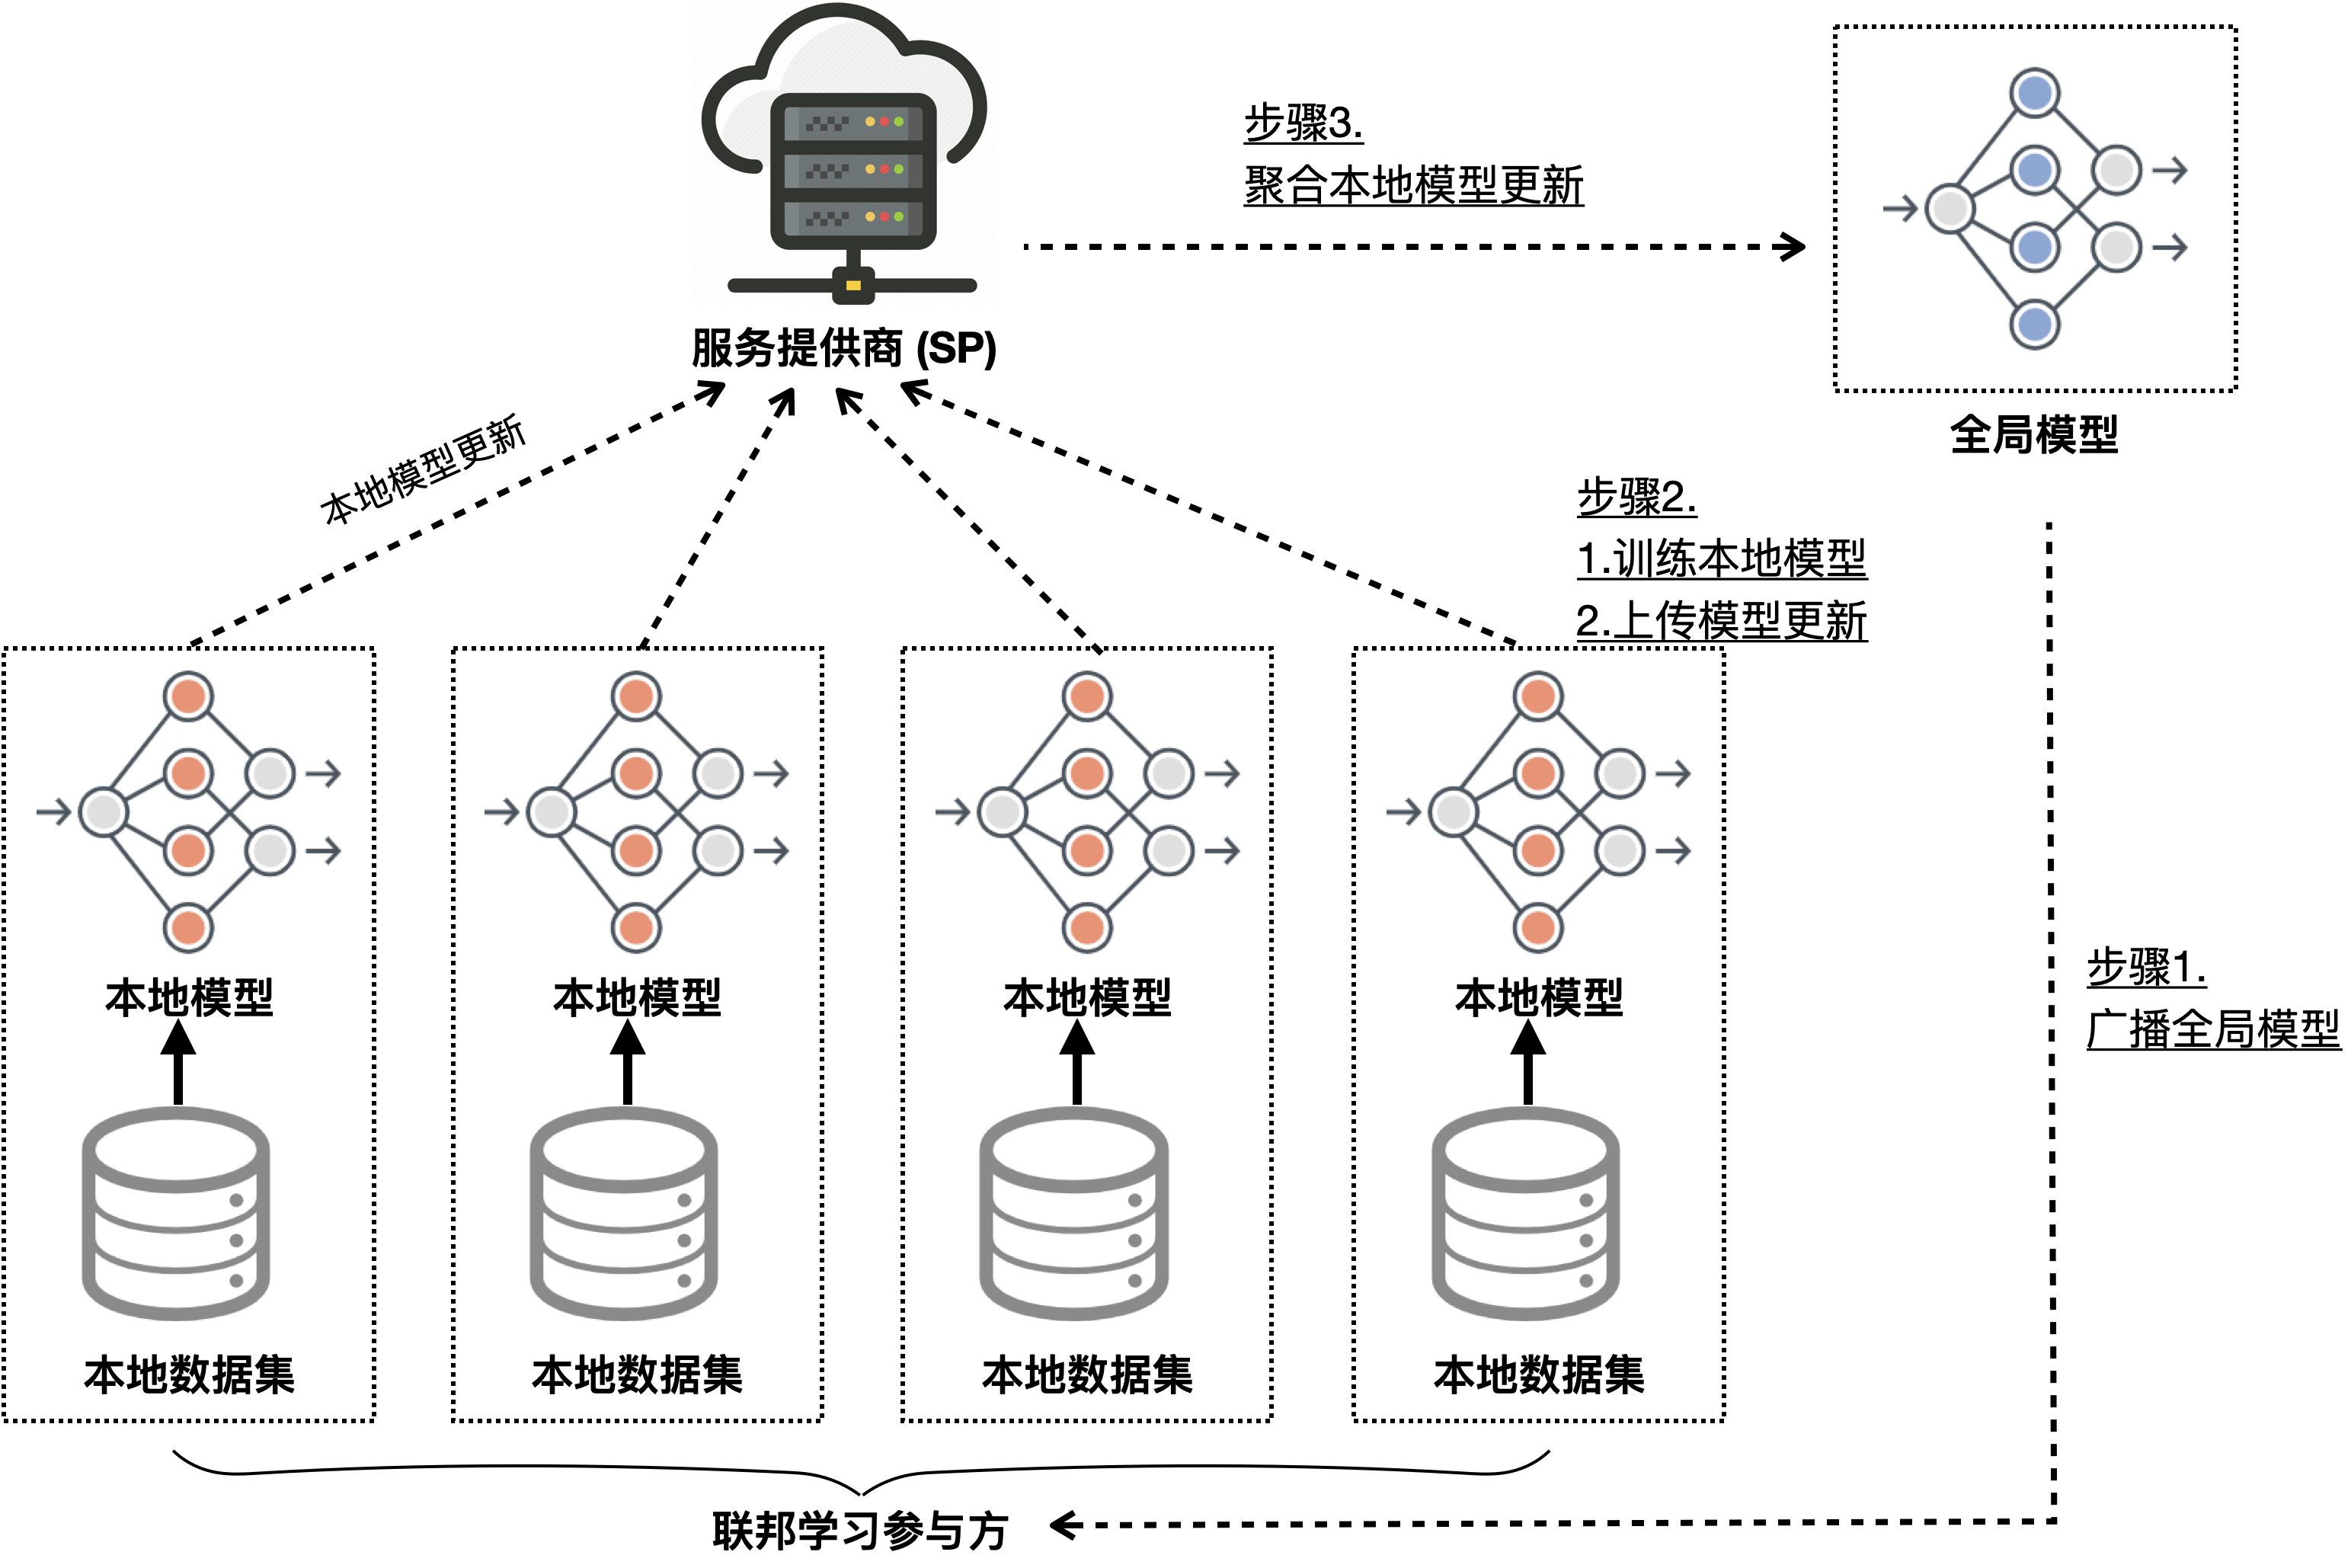
\includegraphics[width=0.8\linewidth]{经典FL}
	\caption{经典联邦学习流程}
	\label{FL}
\end{figure}
\subsubsection{联邦学习概念}
联邦学习的概念首先由Google的学者们在文献\parencite{mcmahan2017communication}中提出,其核心目标是联合各个数据拥有方,在不直接交换数据样本的前提下协同训练出一个全局模型。在联邦学习中,主要有两个角色:(1)持有本地数据的训练参与方;(2)组织整个协同训练过程的服务器。训练过程主要包括以下三个核心步骤(如图\ref{FL}所示):
\begin{compactenum}
	\item \textbf{服务器初始化训练过程:}训练初始化过程主要包括全局模型参数和训练超参数的初始化,超参数主要包括训练轮次、参与方数量以及每轮参与训练的节点占比。全局模型参数初始化完成后,由服务器广播给训练的参与方。
	\item \textbf{参与方训练获取更新后的模型参数:}获取到全局模型参数后,首先将其应用到本地模型,然后使用本地数据进行训练,得到更新后的模型参数(模型权重或梯度),最后将得到的更新信息上传给聚合服务器。
	\item \textbf{服务器聚合得到全局模型:}服务器在收到满足条件的用户模型参数信息后,运行聚合算法生成本轮的全局模型,再分发给参与方进行下一轮的训练。
\end{compactenum}

参与方与服务器重复以上后两个步骤直到满足训练的终止条件,比如达到了最大训练轮次或达到了目标准确率。完成联合训练之后,参与方会获得性能更优的全局模型。

\textbf{讨论:}联邦学习的模型参数信息,具体指的是本地模型更新后的模型权重信息(Model Weights,$W_i$)或更新模型用到的梯度信息(Model Gradients,$G_i$),这两者的聚合在本地学习率和全局学习率一致时是等效的。本文第\ref{pbfl}章方案聚合的模型权重信息,方案描述中的“模型参数”指的是模型权重($W_i$);而本文第\ref{ppfl+hc}章方案聚合的是模型梯度信息,方案描述中的“模型参数”指的是模型梯度($G_i$)。
%TODO 解释一下?
%\footnote{text}

\subsubsection{联邦学习分类}
%%TODO 加图加图!!!
%参考Federated Learning on Non-IID Data: A Survey
根据参与方的样本分布情况,联邦学习分为以下三种类型:横向联邦学习(Horizontal Federated Learning)、纵向联邦学习(Vertical Federated Learning)以及联邦迁移学习(Federated Transfer Learning)\cite{zhu2021fedsurvey}。三种类型的联邦学习样本分布示例如图\ref{fldemo}所示。
\begin{figure}
	\centering%
	\subfloat[横向联邦学习示例]{%
		\label{fldemo:hfl}
		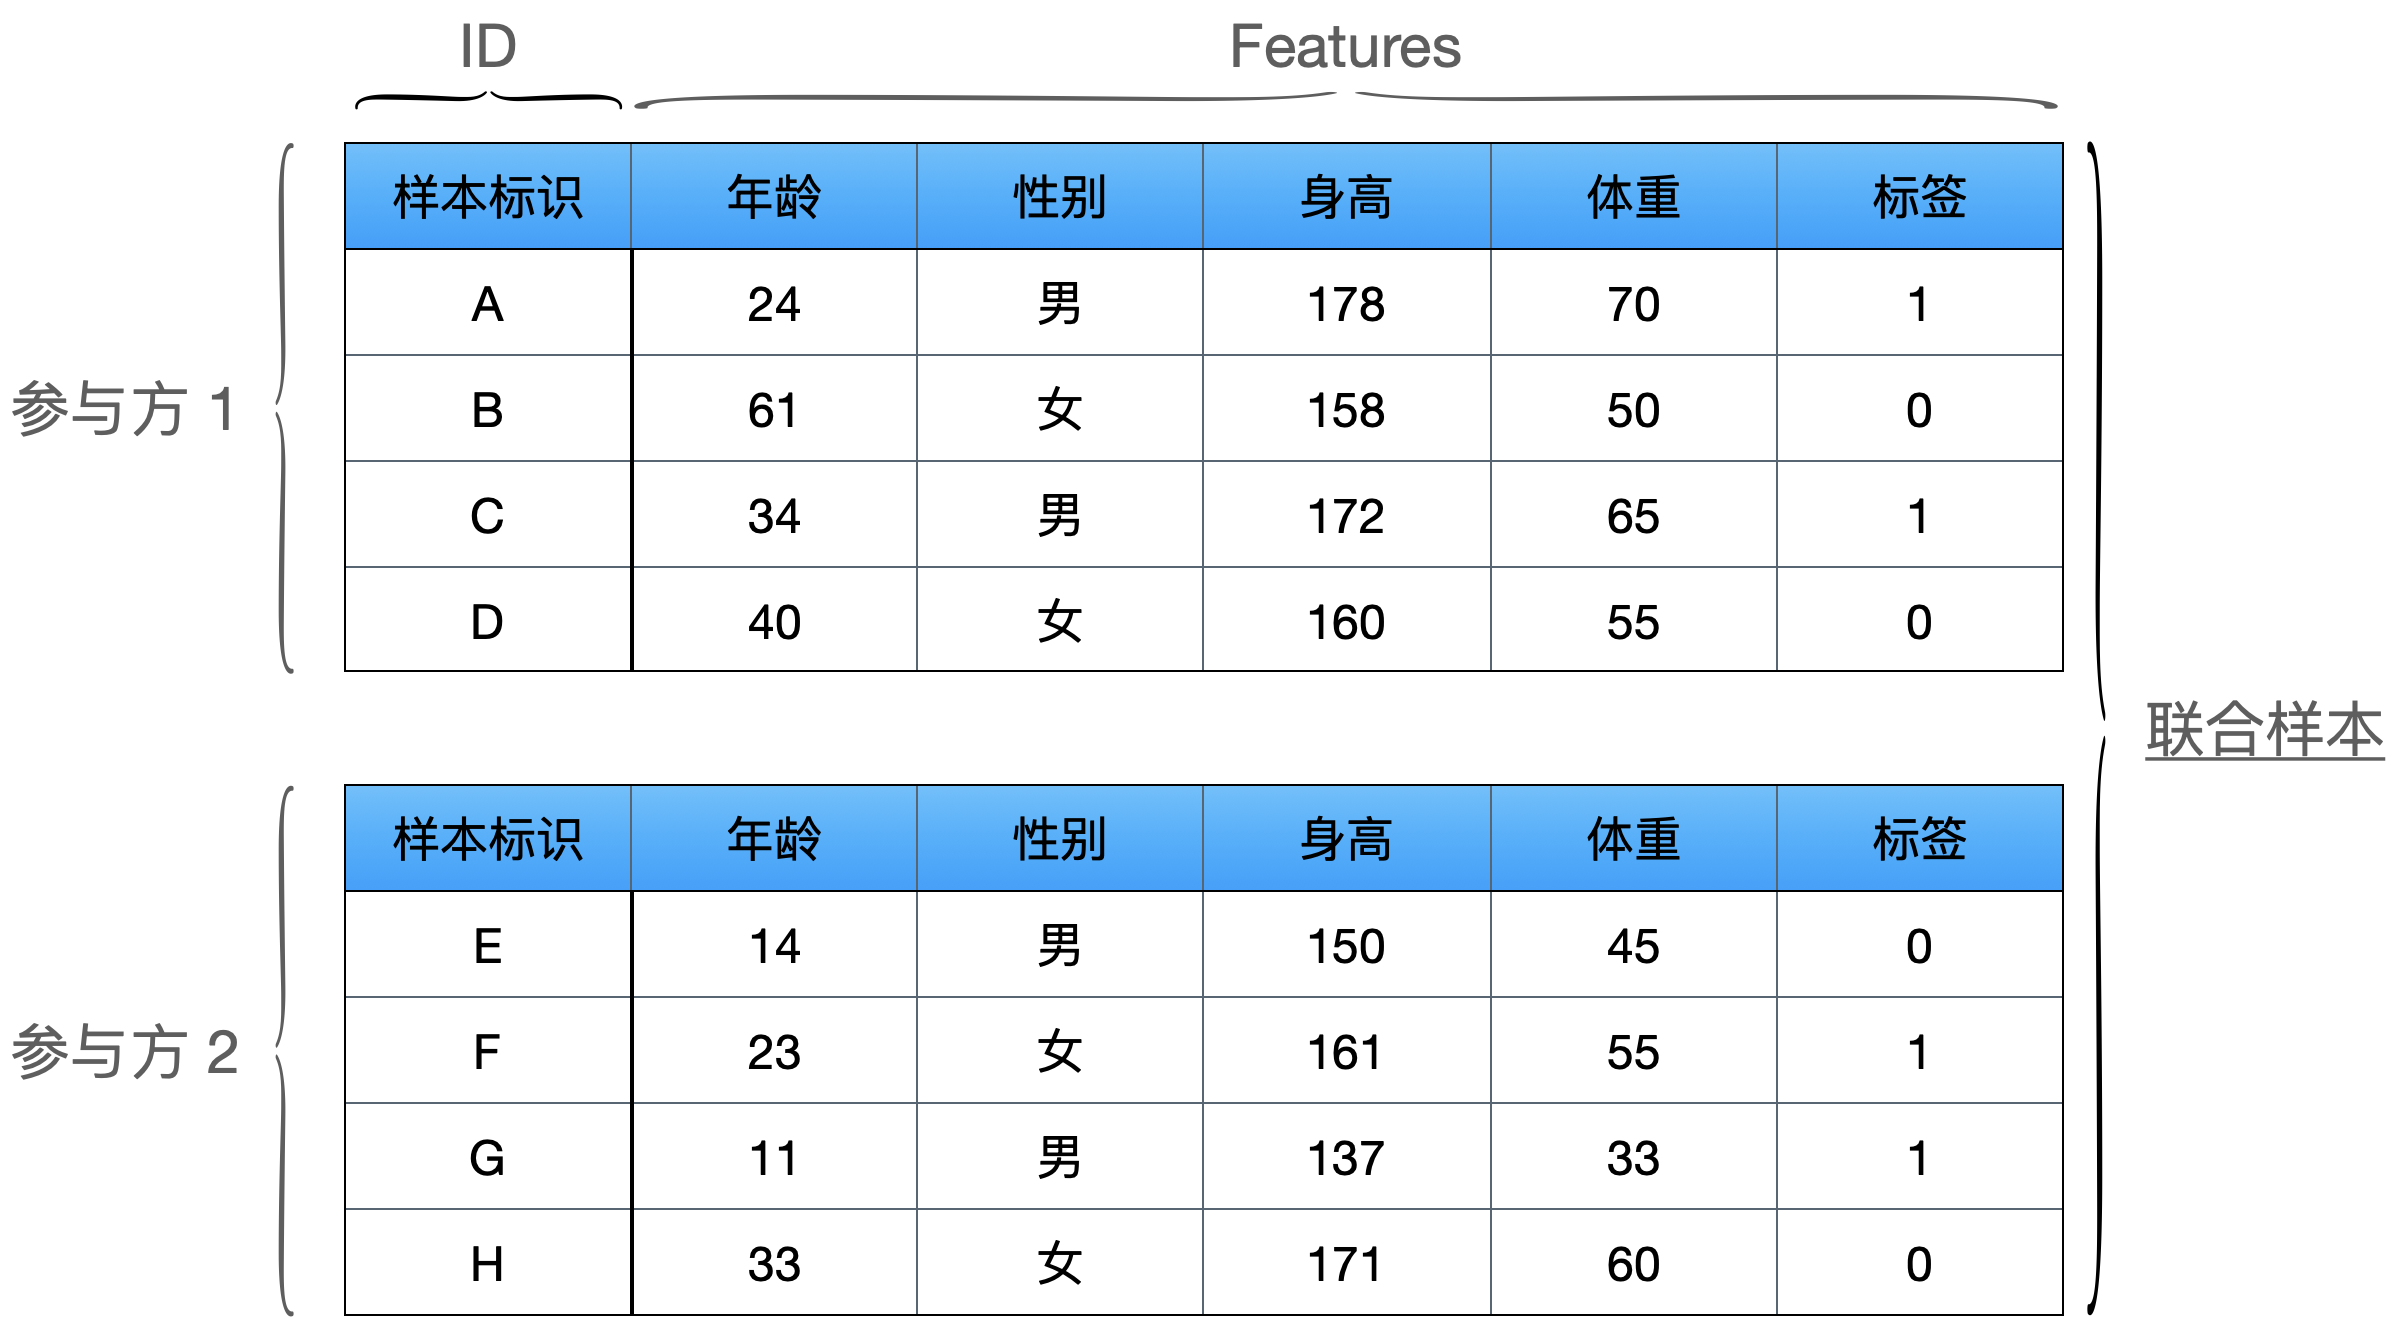
\includegraphics[width=0.5\linewidth]{横向联邦学习-noalpha}}%\hspace{4em}%
	\subfloat[纵向联邦学习示例]{%
		\label{fldemo:vfl}
		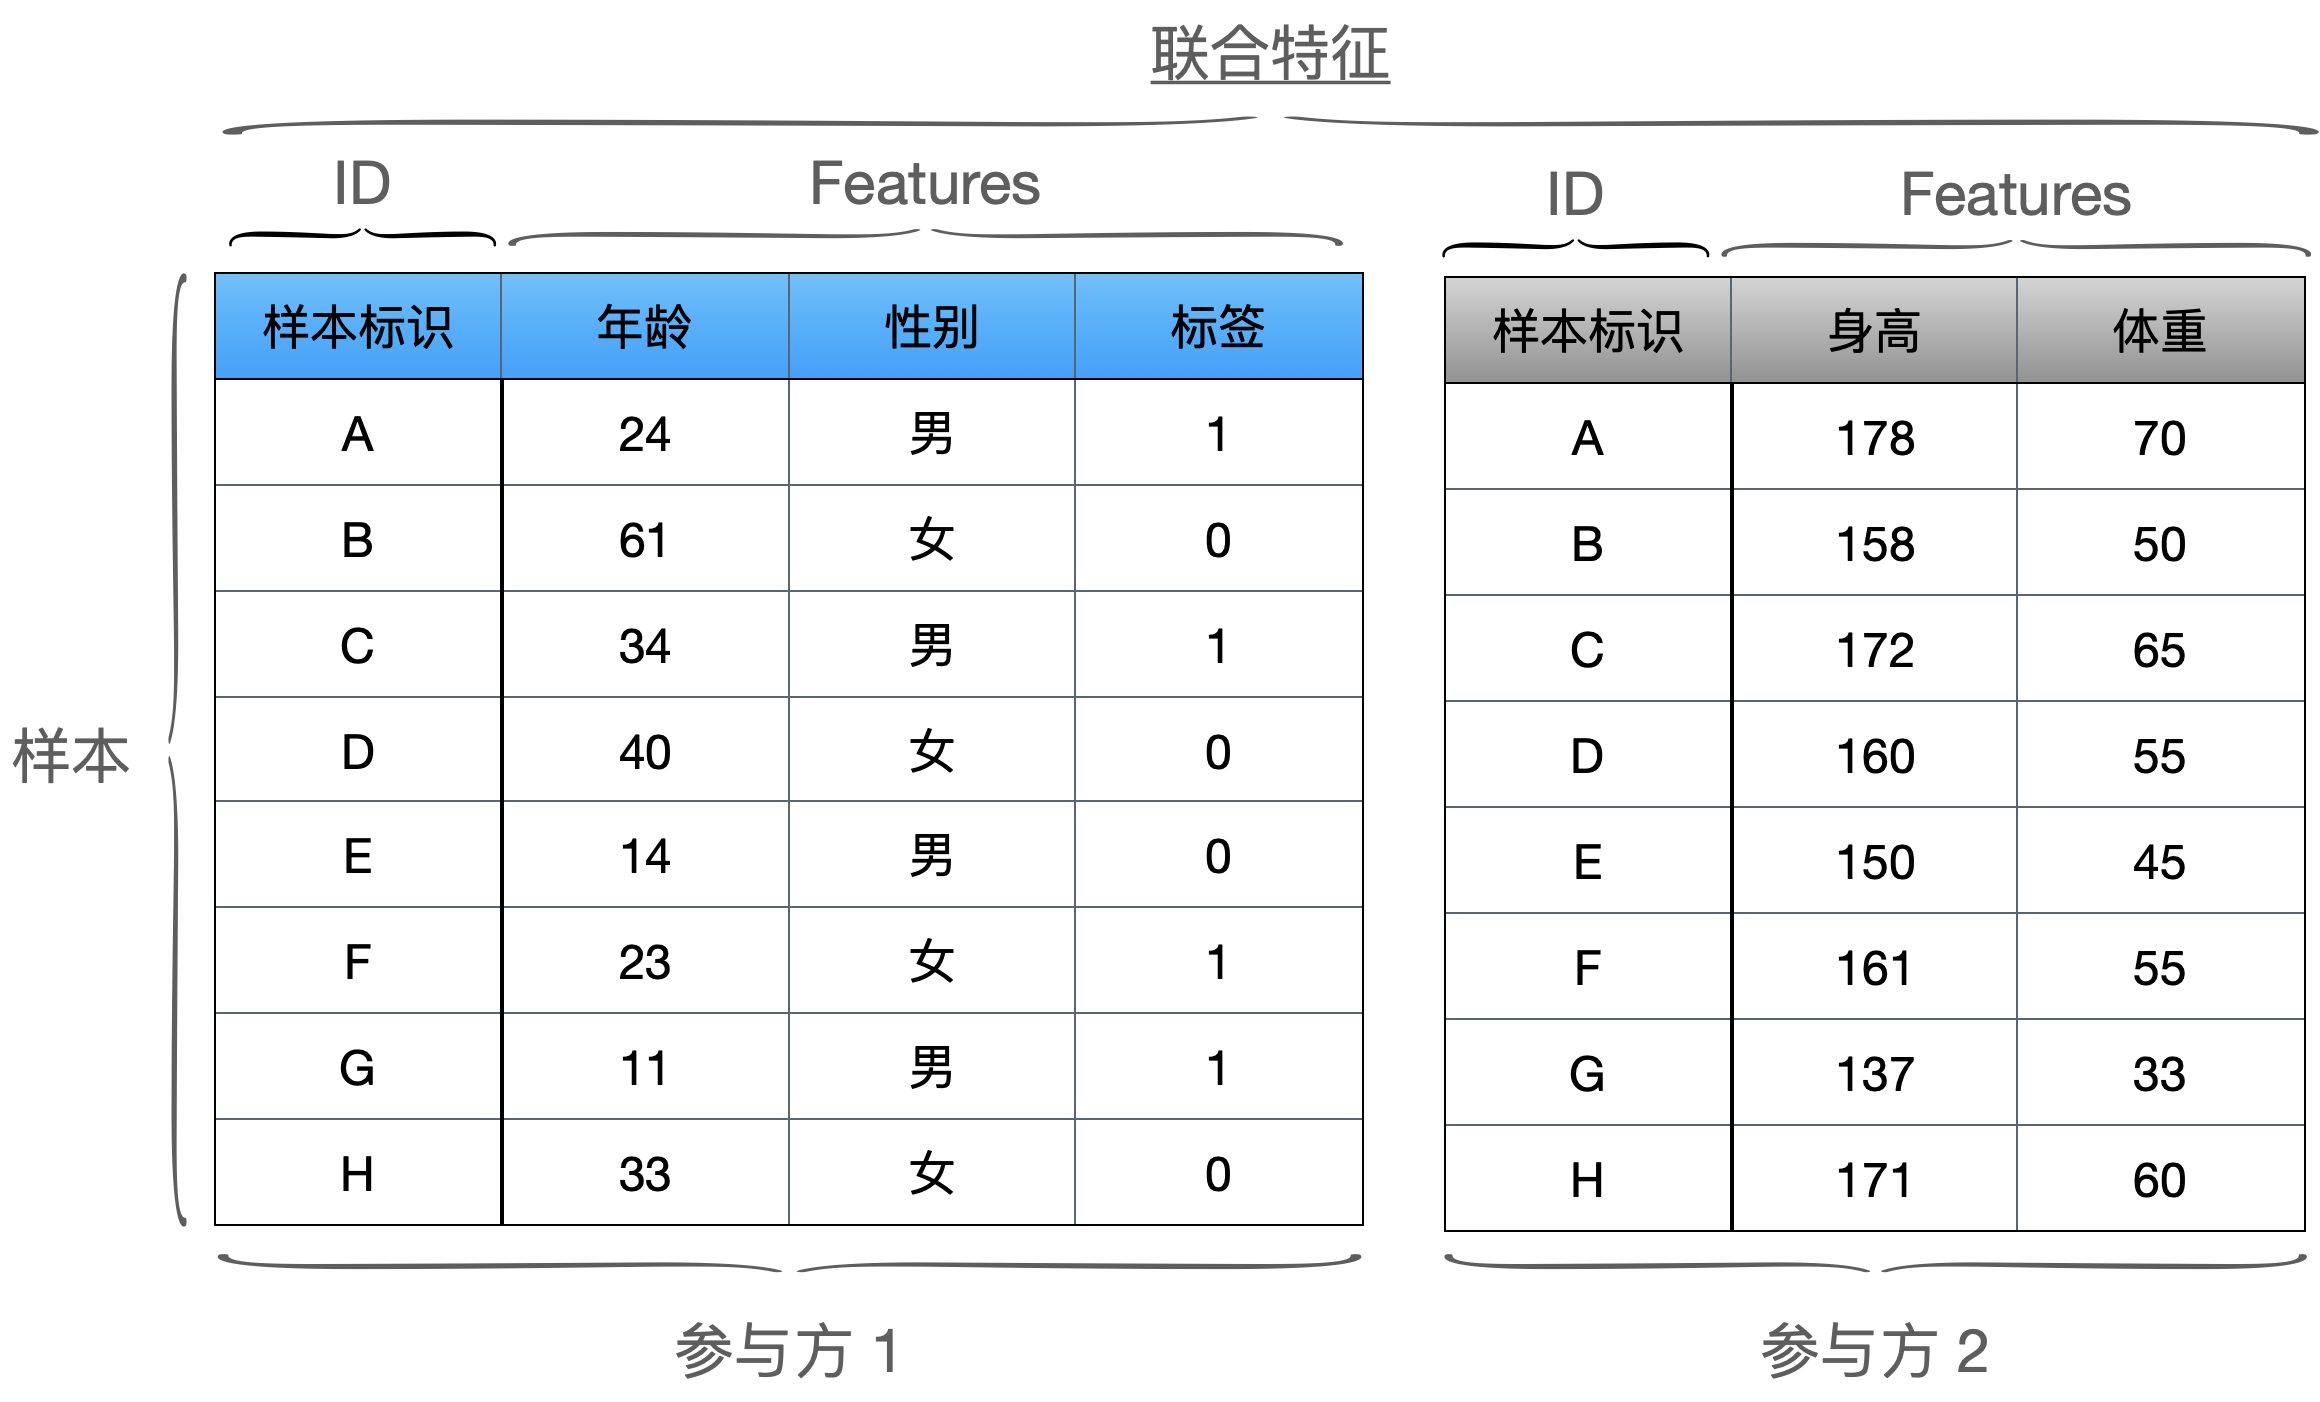
\includegraphics[width=0.5\linewidth]{纵向联邦学习-noalpha}} \\
	\subfloat[联邦迁移学习示例]{
		\label{fldemo:ftl}
		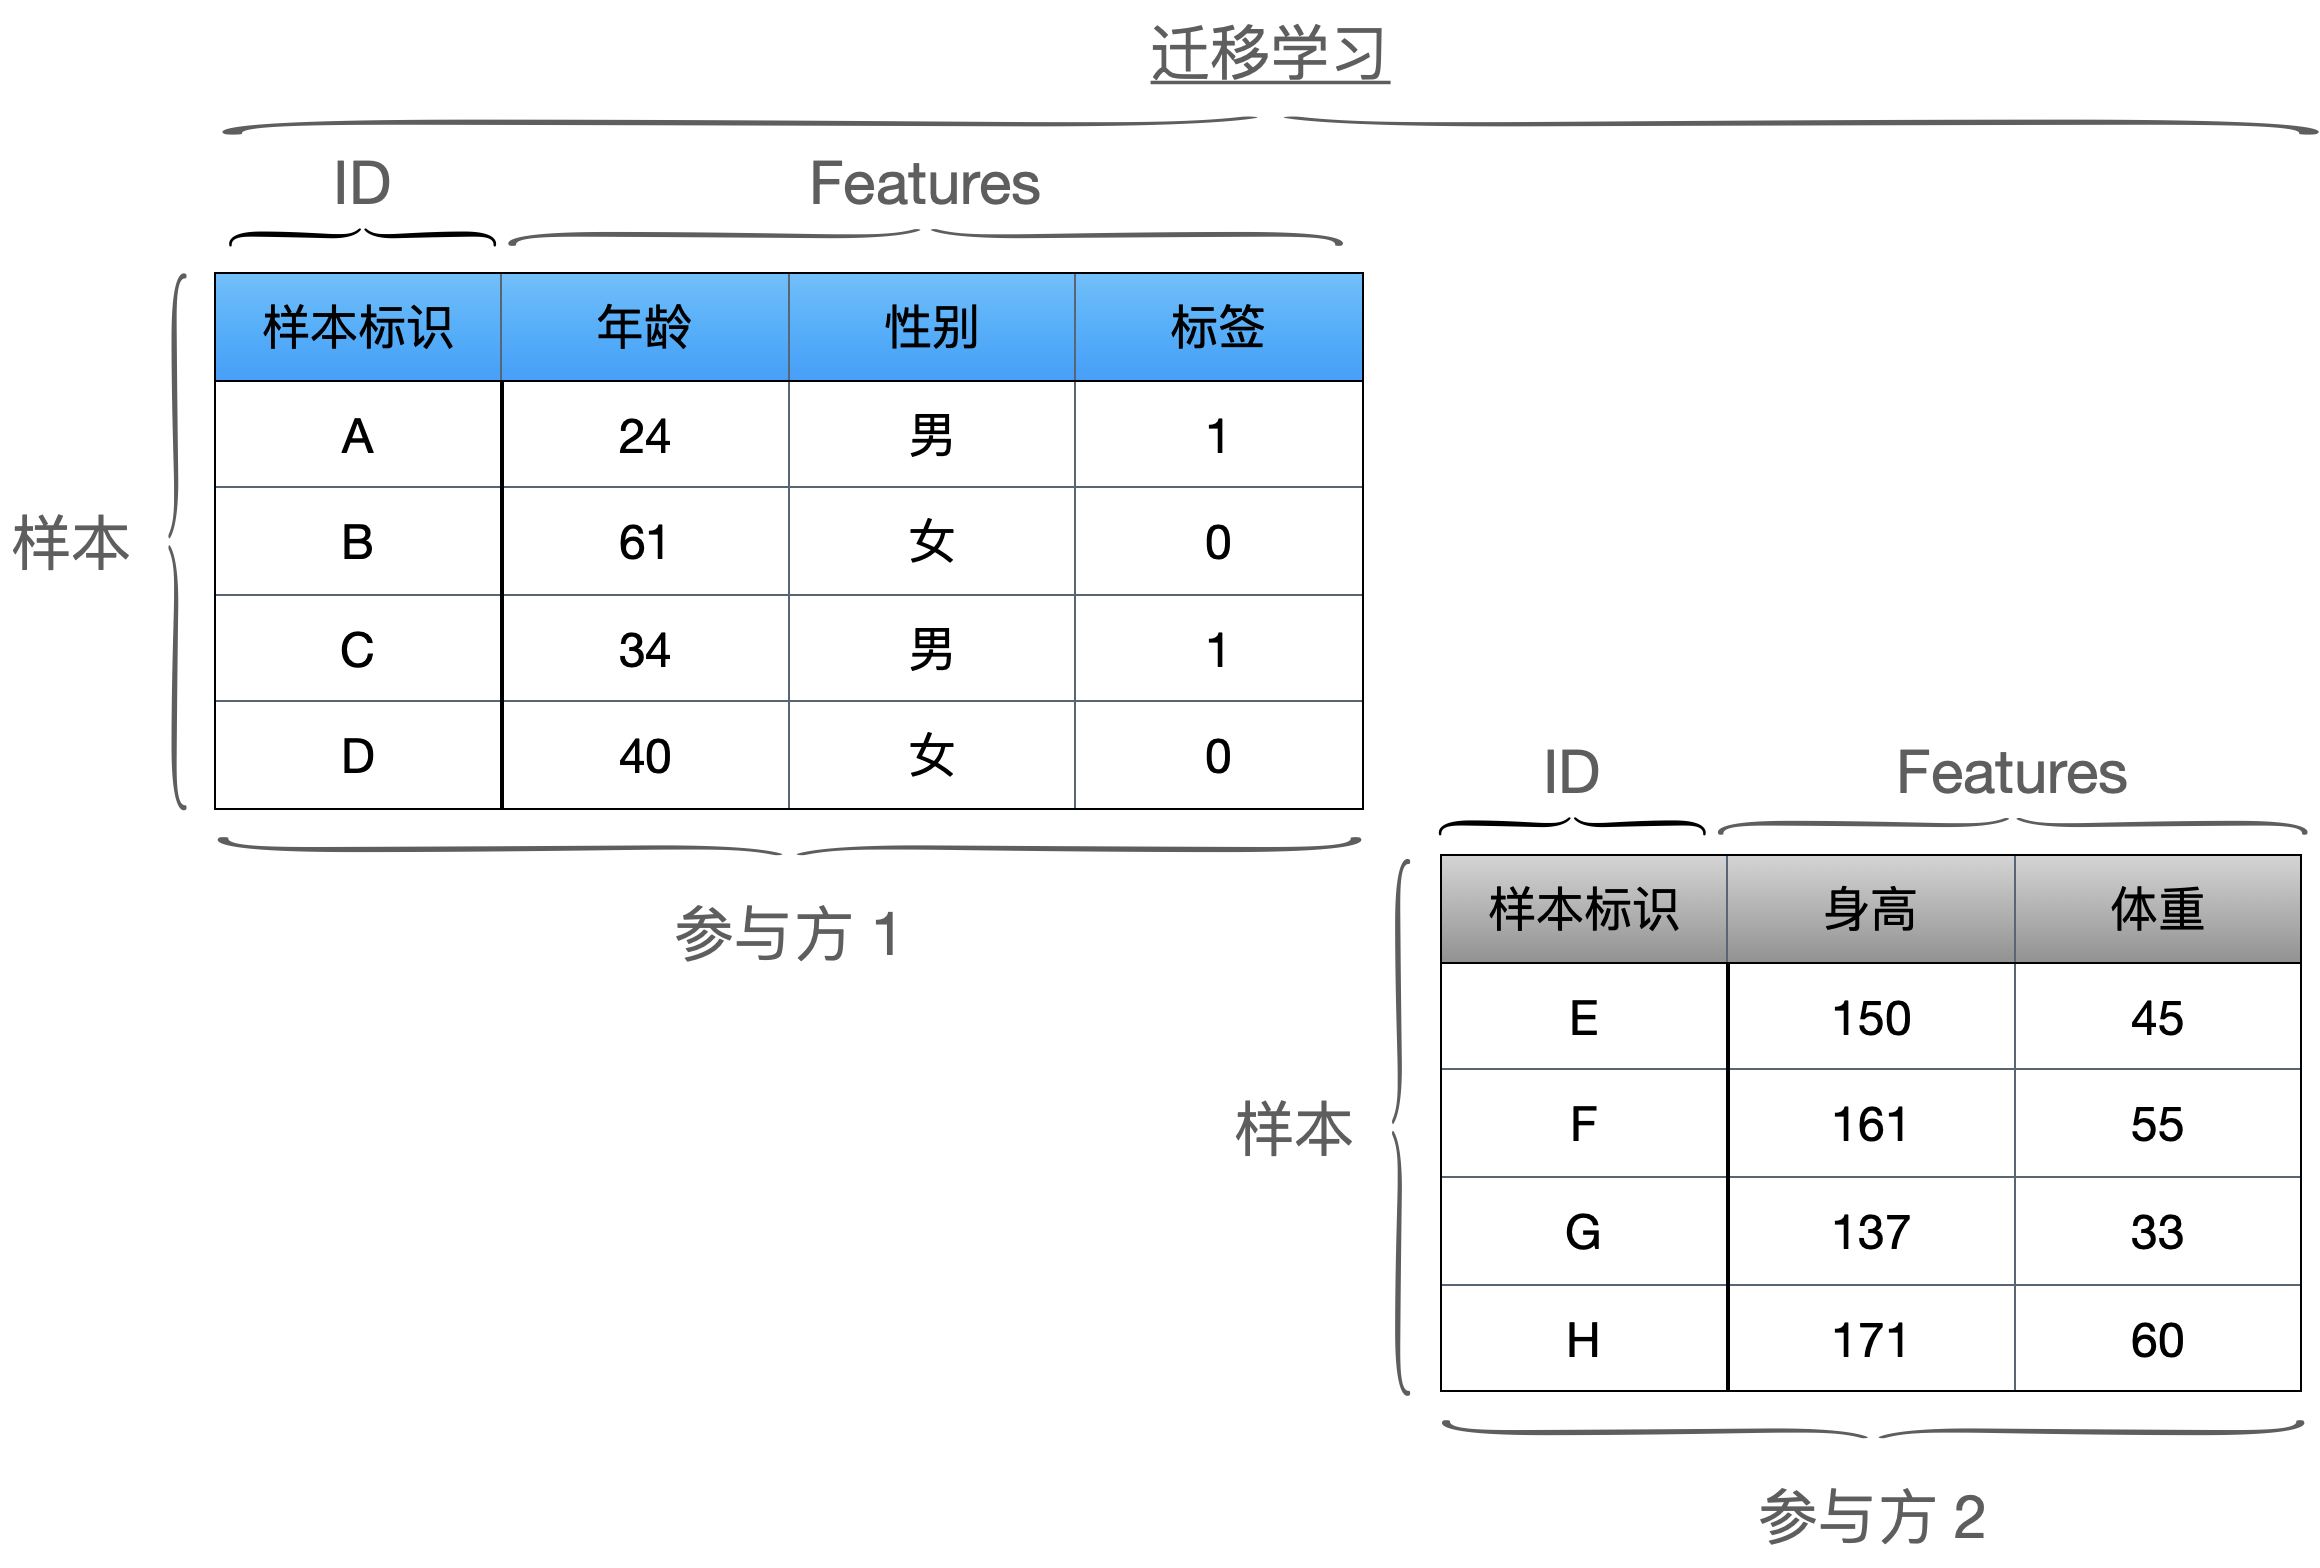
\includegraphics[width=0.5\linewidth]{迁移联邦学习-noalpha}}
	\caption{联邦学习分类示例}
	\label{fldemo}
\end{figure}

为了更清晰的描述这三者的特点,本小节首先给出如下形式化描述:${D}_i$ 表示参与方$i$的本地数据集,其中$d \in {D}_i$ 是其中的一个样本,假设样本$d$由三部分构成,即$d = (d_{ID}, d_{feature}, d_{label}), d_{ID} \in \mathcal{X}^i_{ID}, d_{feature} \in \mathcal{X}^i_{feature}, d_{label} \in \mathcal{X}^i_{label}$,其中$\mathcal{X}^i_{ID}, \mathcal{X}^i_{feature}, \mathcal{X}^i_{label}$分别表示参与方$i$持有数据集${D}_i$的样本标识空间、特征空间和标签空间。基于不同参与方的样本标识空间$\mathcal{X}_{ID}$和特征空间$\mathcal{X}_{feature}$之间的关系,可以将联邦学习划分为横向联邦学习、纵向联邦学习和联邦迁移学习。

%\begin{figure}[ht]
%	\centering
%	\begin{minipage}[b]{0.45\linewidth}
%		\centering
%		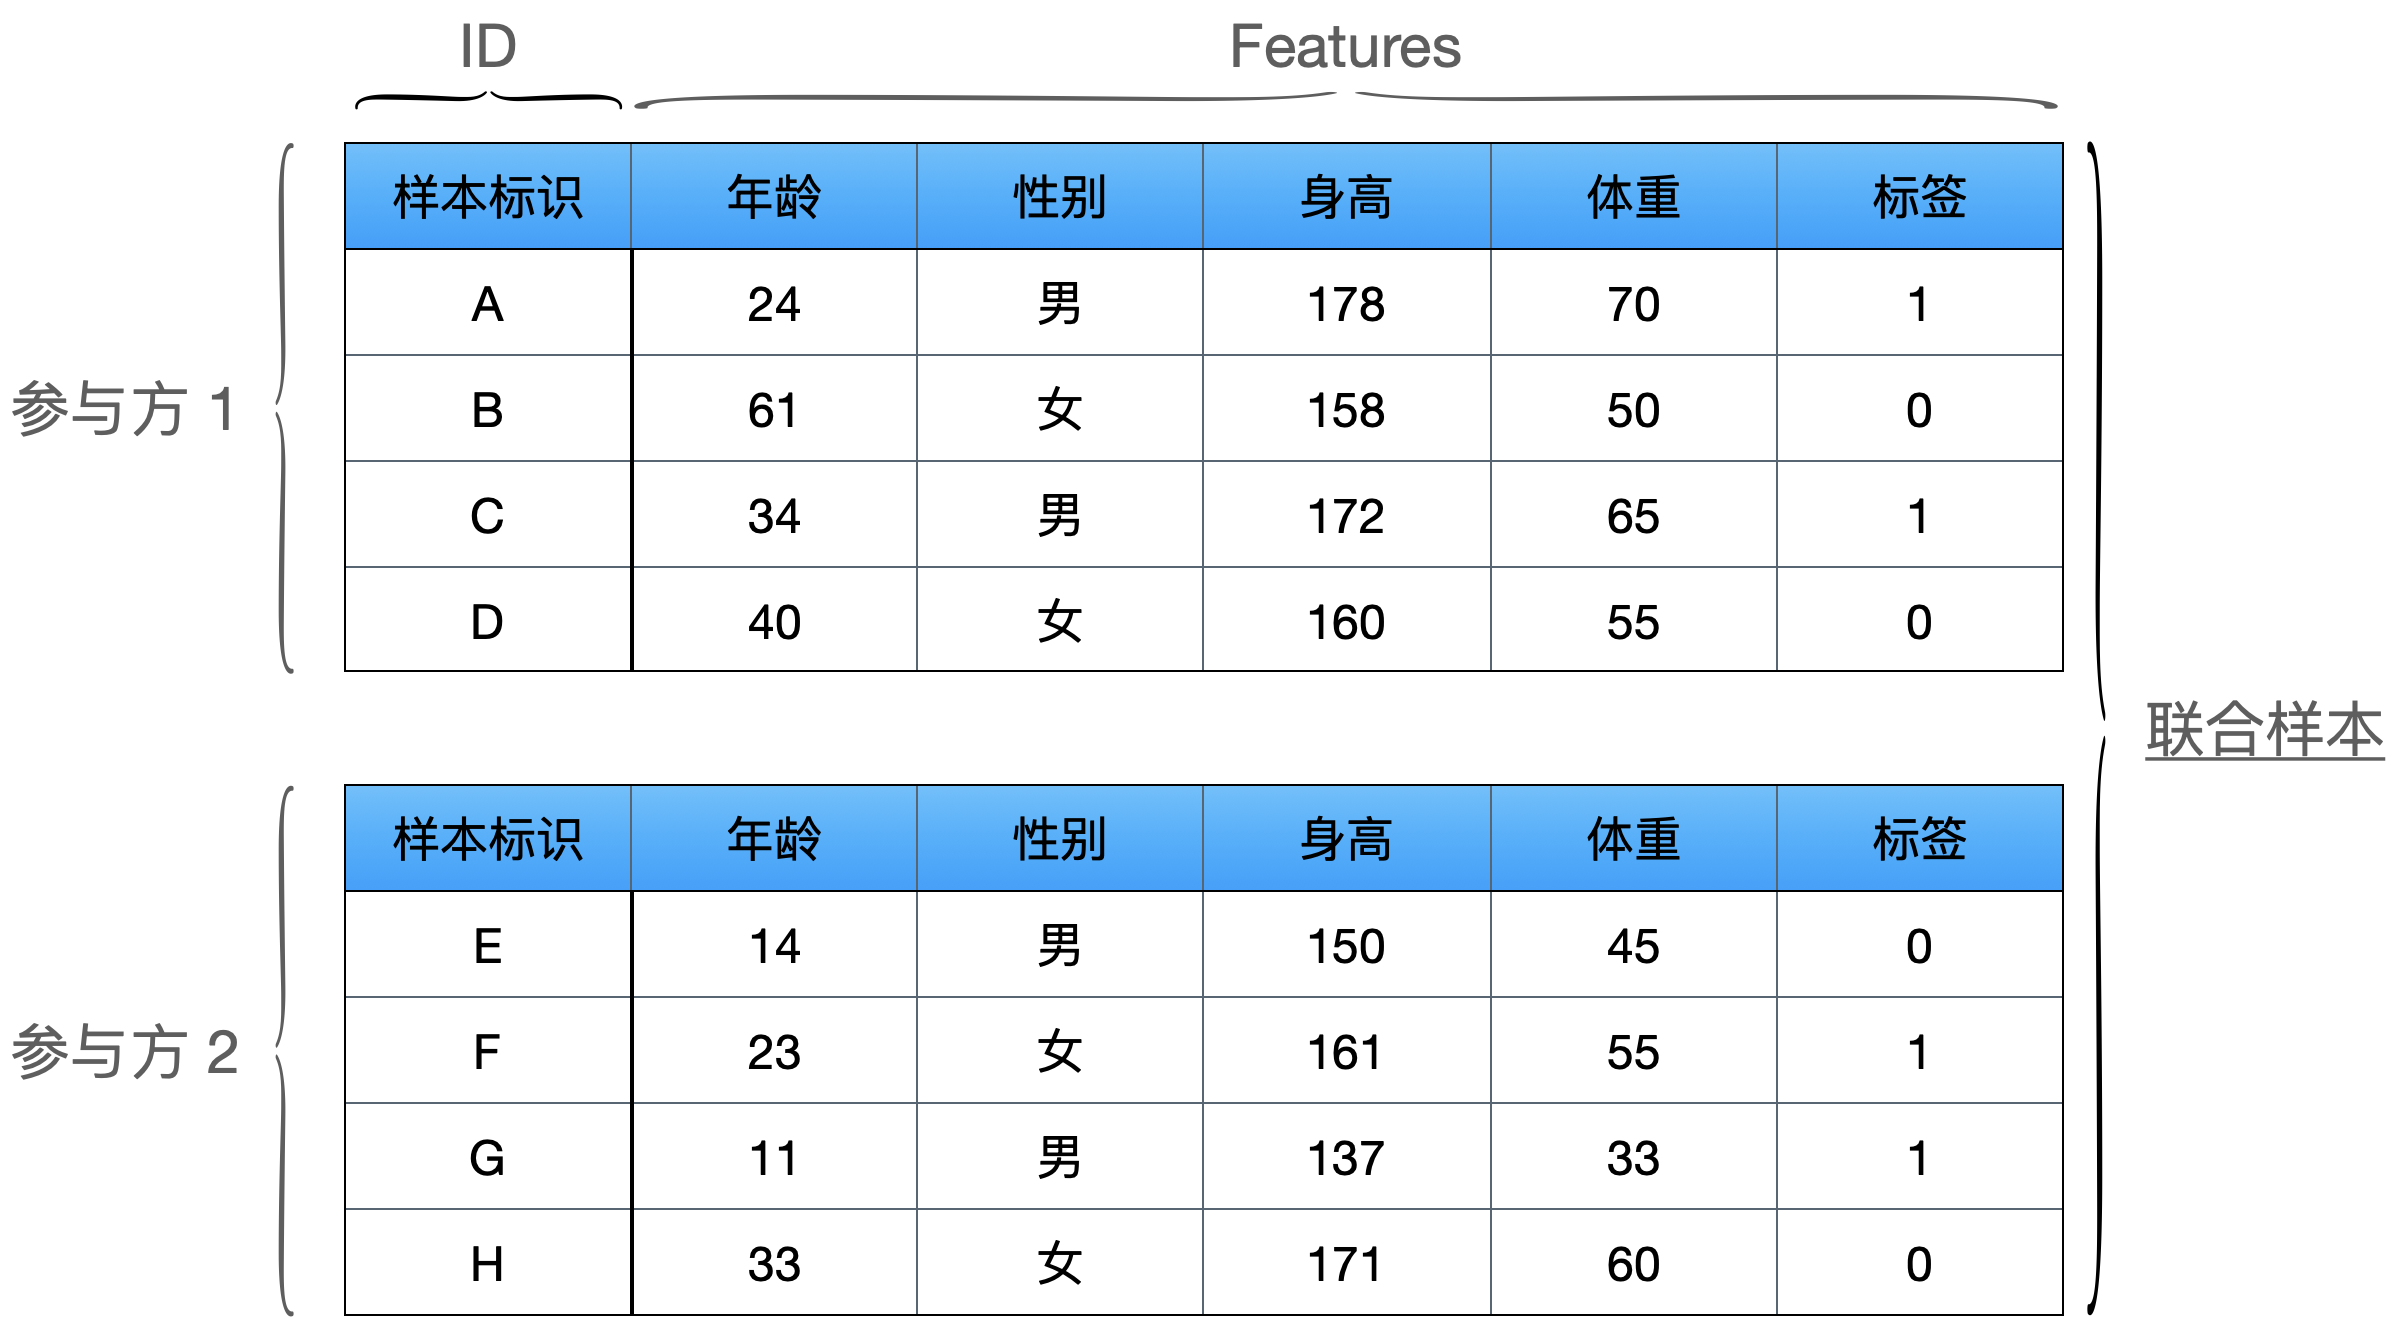
\includegraphics[width=\linewidth]{横向联邦学习-noalpha}
%		\caption{横向联邦学习示例}
%		\label{fldemo:hfl}
%	\end{minipage}
%	\hspace{0.5cm}
%	\begin{minipage}[b]{0.45\linewidth}
%		\centering
%		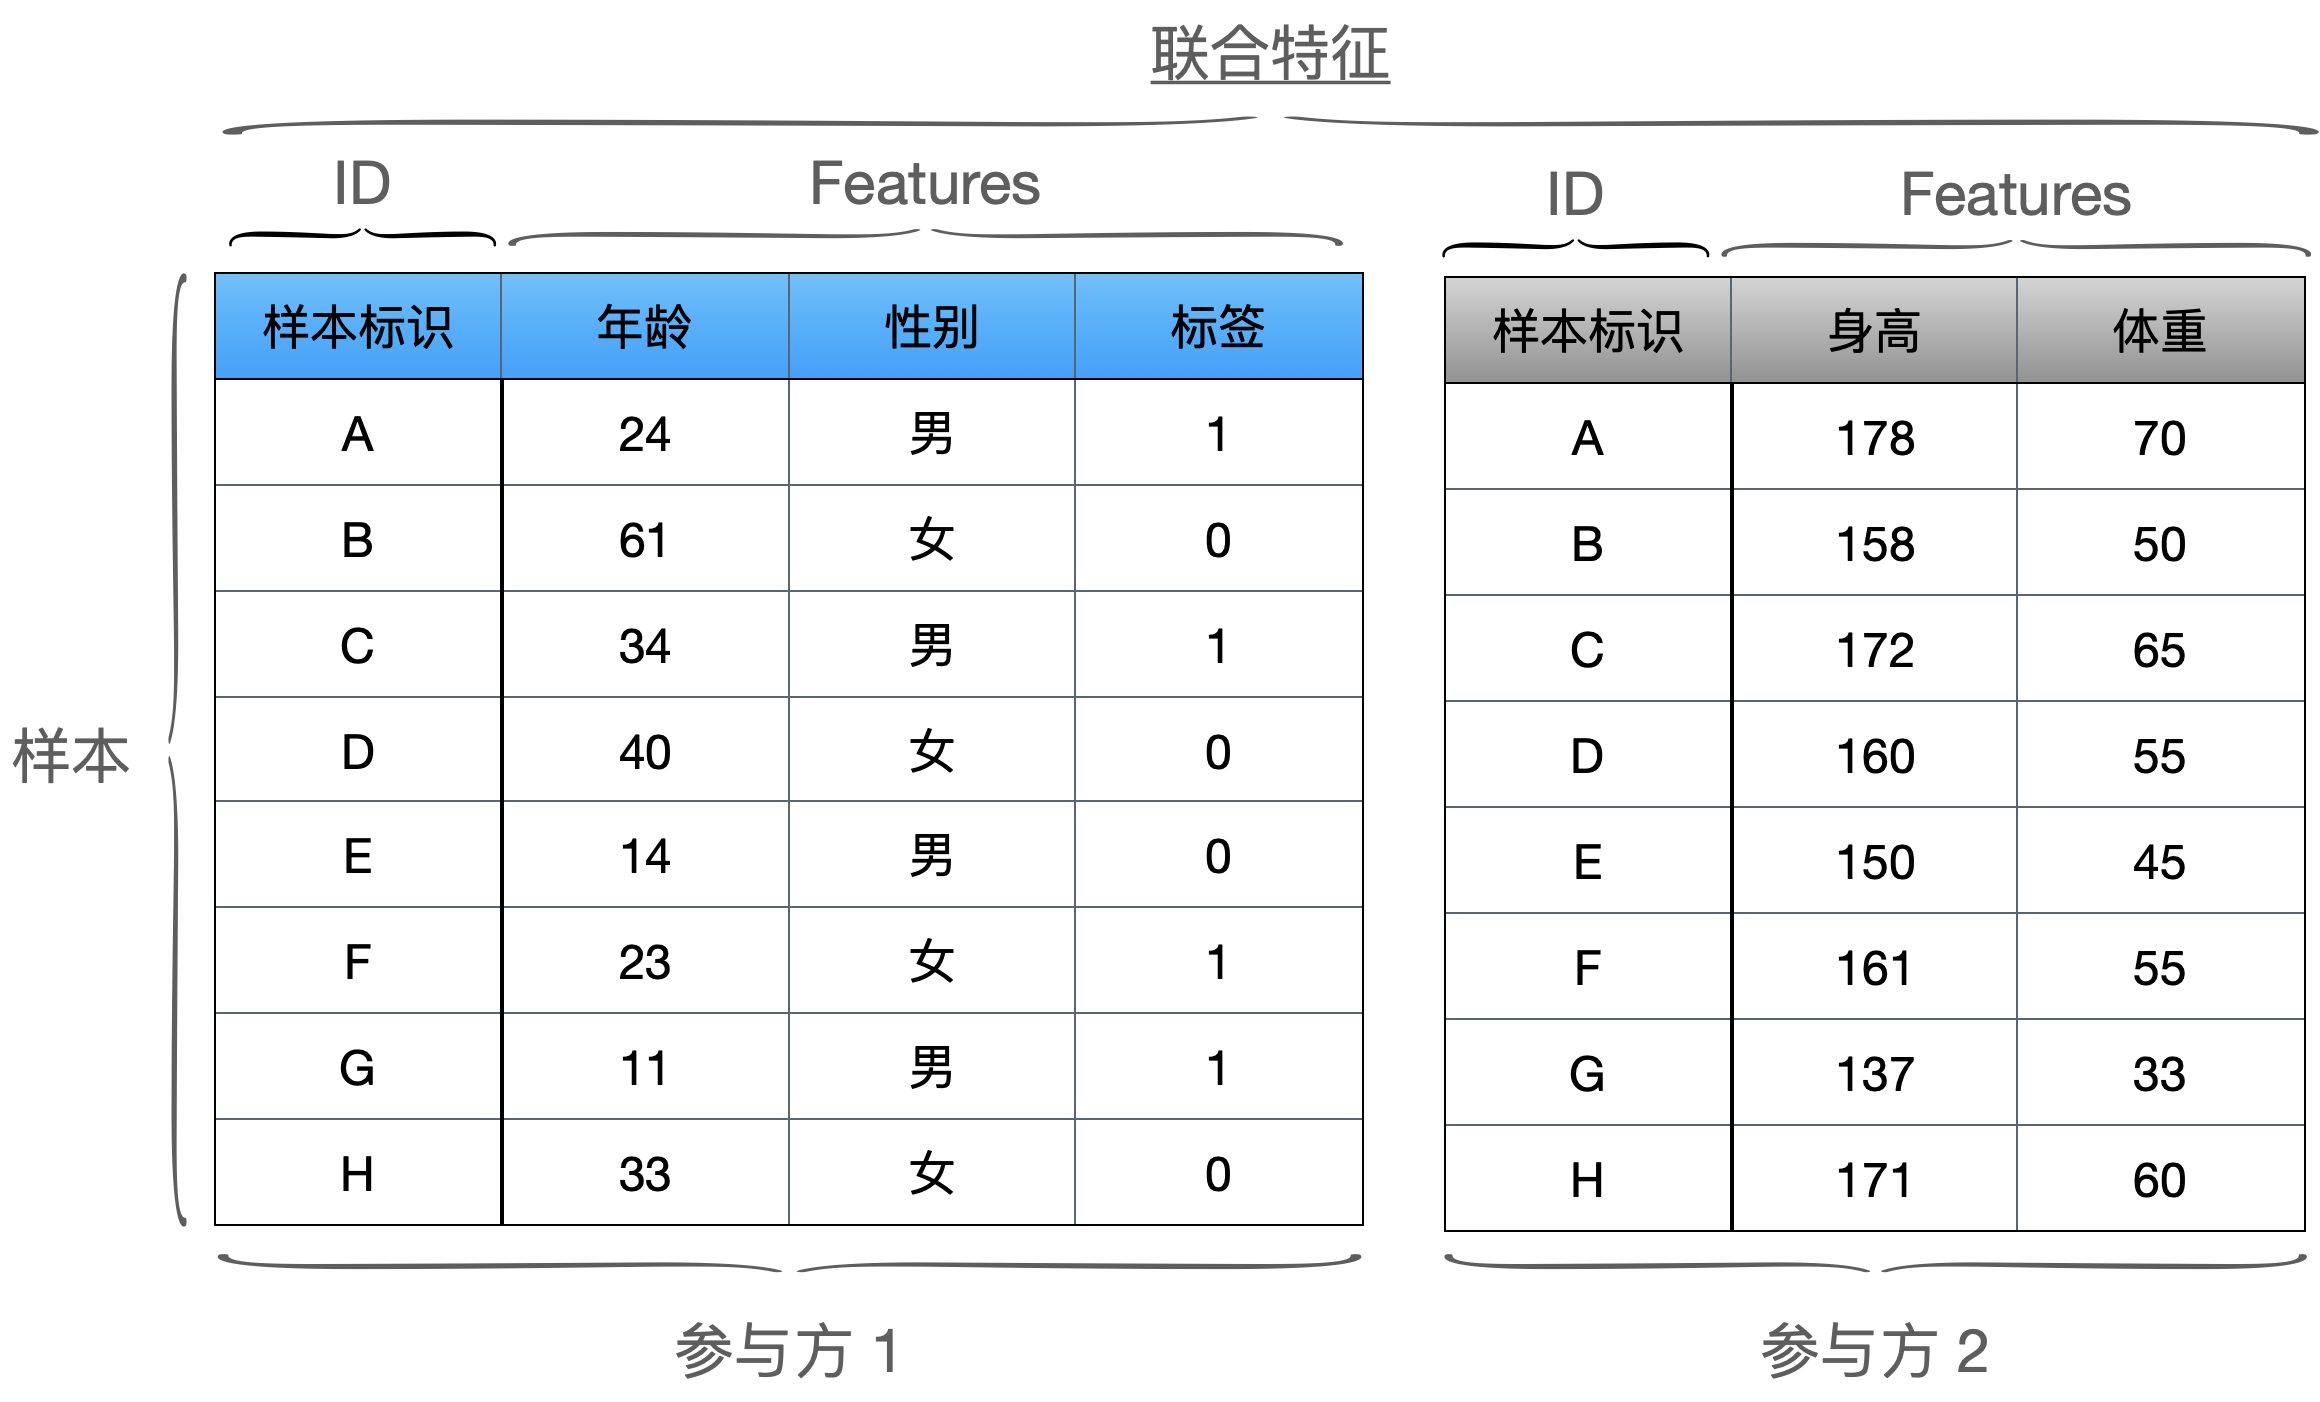
\includegraphics[width=\linewidth]{纵向联邦学习-noalpha}
%		\caption{纵向联邦学习示例}
%		\label{fldemo:vfl}
%	\end{minipage}
%
%
%	\begin{minipage}[b]{0.45\linewidth}
%		\centering
%		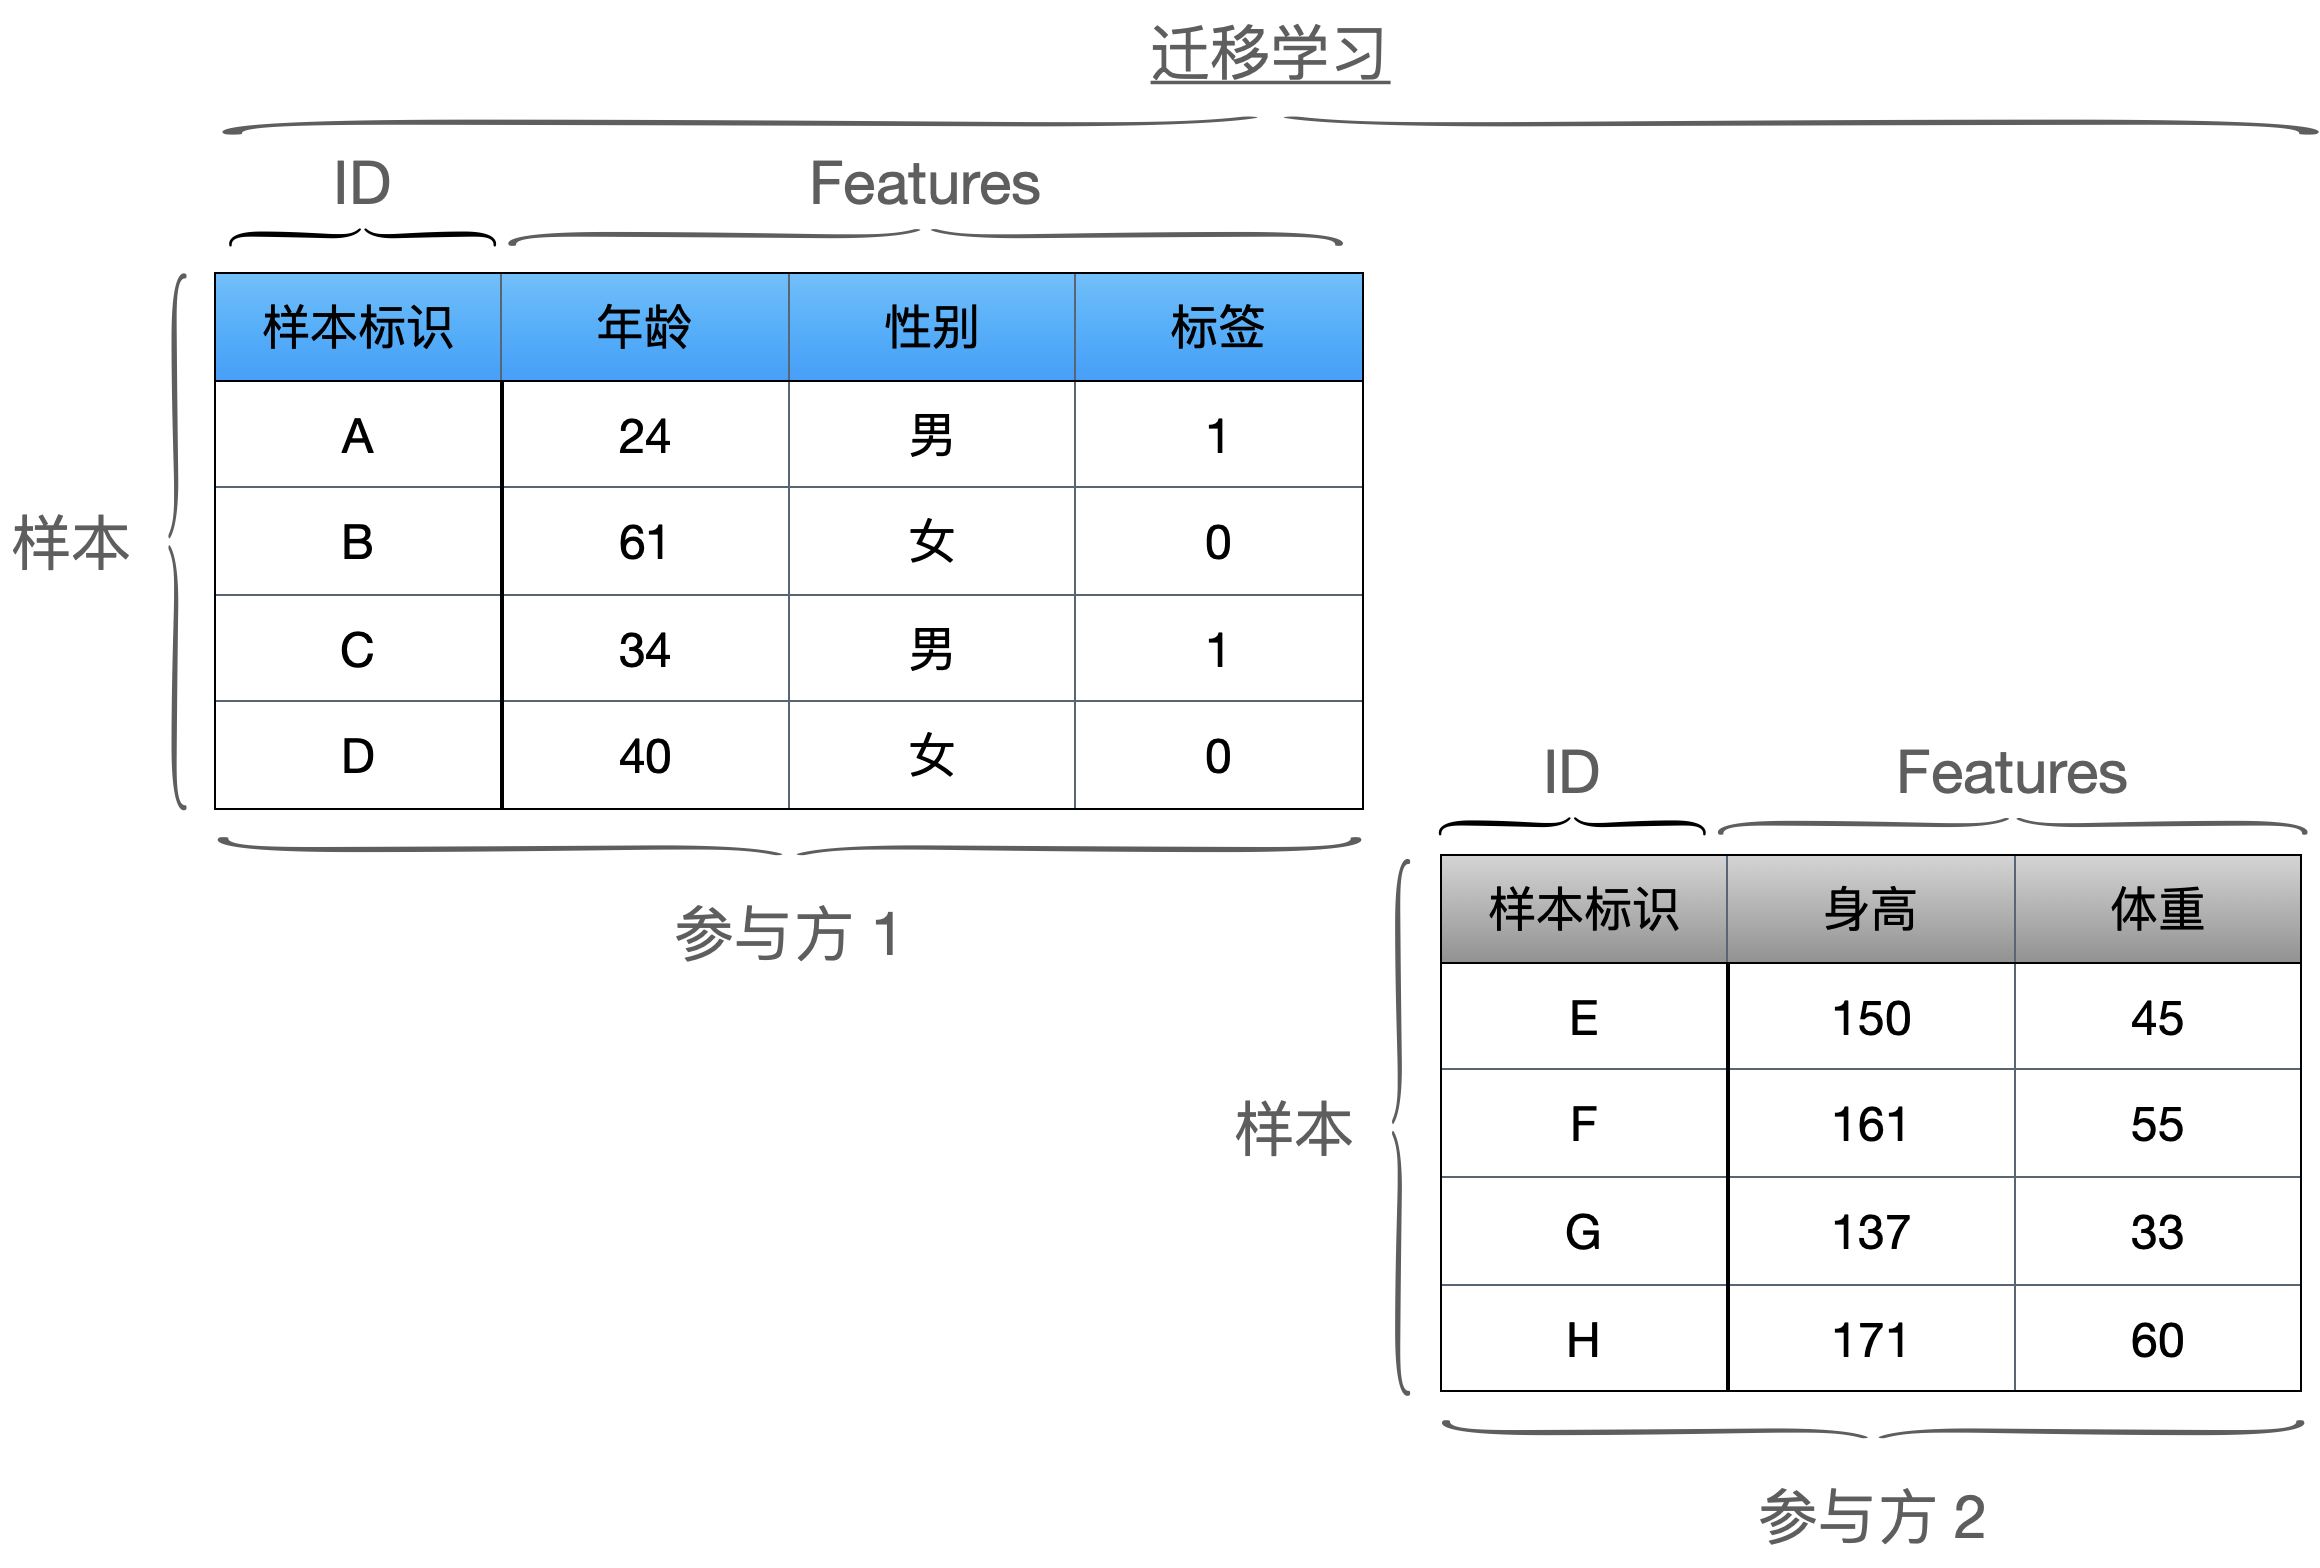
\includegraphics[width=\linewidth]{迁移联邦学习-noalpha}
%		\caption{迁移联邦学习示例}
%		\label{fldemo:ftl}
%	\end{minipage}
%%	\caption{Three images side by side.}
%%	\label{fig:three_images}
%\end{figure}

(1)横向联邦学习:参与方之间的样本标识空间($\mathcal{X}_{ID}$)不同,而特征空间($\mathcal{X}_{feature}$)相同,即:
\begin{equation}
	\mathcal{X}_{ID}^i \neq \mathcal{X}_{ID}^j, \mathcal{X}_{feature}^i=\mathcal{X}_{feature}^j , \forall {D}_i, {D}_j, i \neq j
\end{equation}
例如,不同城市的几个医院之间,掌握着不同的病人($\mathcal{X}_{ID}$不同)的数据,而由于相似的数据获取标准,每个病人数据样本中的属性相同($\mathcal{X}_{feature}$相同)。
图\ref{fldemo:hfl}中描述的是典型的横向联邦学习所面临的数据分布,其本质上是对不同参与方在样本数量上的联合。
Mcmahan等人\cite{mcmahan2017communication}最先提出的联邦学习就是典型的横向联邦学习,其优点是可以增加参与训练的样本数量。

(2)纵向联邦学习:参与方之间的样本标识空间($\mathcal{X}_{ID}$)相同,而特征空间($\mathcal{X}_{feature}$)不同,即:
\begin{equation}
	\mathcal{X}_{ID}^i = \mathcal{X}_{ID}^j, \mathcal{X}_{feature}^i \neq \mathcal{X}_{feature}^j , \forall {D}_i, {D}_j, i \neq j
\end{equation}
例如,同一个城市的医院和银行都接纳过相同的客户($\mathcal{X}_{ID}$相同),但是医院和银行记录的用户相关数据的属性不一致($\mathcal{X}_{feature}$不同)。这种情况下医院和银行之间的数据在样本ID上是重合的,但是拥有的属性完全不同。
在训练时首先要对样本ID进行对齐,然后在本地训练并分享模型参数。
图\ref{fldemo:vfl}中描述的是典型的纵向联邦学习所面临的数据分布,它本质上是对不同参与方数据特征的联合。

(3)联邦迁移学习:参与方之间的样本标识空间($\mathcal{X}_{ID}$)与特征空间($\mathcal{X}_{feature}$)都不同,即:
\begin{equation}
	\mathcal{X}_{ID}^i \neq \mathcal{X}_{ID}^j, \mathcal{X}_{feature}^i \neq \mathcal{X}_{feature}^j , \forall {D}_i, {D}_j, i \neq j
\end{equation}
针对这种样本和特征重叠都比较少的情形,迁移学习被引入了进来,它能够将相关领域的知识迁移到目标领域,弥补数据分布上的差异,使得参与方协同学习迁移知识。
图\ref{fldemo:ftl}描述了典型的联邦迁移学习所面临的数据分布,借助于迁移学习联合样本和特征都不同的数据协同训练。

本文的研究对象是由Mcmahan等人\cite{mcmahan2017communication}提出的横向联邦学习,为了简化表述,下文中出现的联邦学习(FL)关键字,指的都是横向联邦学习场景。

\subsection{联邦学习中的隐私威胁}
尽管联邦学习没有直接获取用户的隐私数据,但其中间交换的参数仍然面临着泄露隐私的风险,本小节首先介绍隐私泄露风险来源,然后阐述常见的隐私攻击策略。

\subsubsection{隐私风险来源}
%TODO 可以加表格
联邦学习模型参数的交易发生在两个阶段,即模型参数的上传与下发阶段,这两个阶段都有隐私泄露的风险,下面详细阐述:
\begin{compactitem}
	\item \textbf{模型参数上传阶段:}参与方在完成本地训练之后,将本地更新得到的参数上传给聚合服务器。本阶段潜在的攻击者是聚合服务器,半诚实的服务器可以对收集到的参数发起数据重构攻击,还原用户隐私数据;或者成员推断攻击,推测某个已知样本是否在参与方的训练集中。例如对疾病数据的联合训练,服务器可以探测某个病人是否出现在训练集,进而判断是否患有此种疾病。
	\item \textbf{模型参数下发阶段:}聚合服务器完成对参与方参数的聚合之后,得到了全局模型参数,再将其分发给参与方进行下一轮的训练。本阶段的潜在攻击者可以是恶意的参与方和聚合服务器,同样可以发起数据重构攻击和成员推断攻击,来获取其它参与方的数据隐私。
\end{compactitem}

\subsubsection{常见隐私攻击策略}
在联邦学习中常见的隐私攻击策略有两种,数据重构攻击和成员推断攻击,接下来对这两种攻击进行详细的介绍。

(1)数据重构攻击:由Zhu等人\cite{zhu2019deep}的梯度深度泄露算法(Deep Leak from Gradients,DLG),展示了从用户梯度恢复出用户数据样本的方法。攻击者只需要获取特定参与方的一轮训练梯度,提供随机输入值,然后迭代优化随机值,使得生成的梯度与目标梯度类似,经过优化的输入值就是生成的近似样本。以随机样本$(\mathtt{x}^{\prime}_1, \mathtt{y}^{\prime}_1)$为例,其中$\mathtt{x}^{\prime}_1$和$\mathtt{y}^{\prime}_1$分别表示样本特征和标签,通过模型计算得到生成的模拟梯度$\nabla W^{\prime}_i$,然后以该梯度$\nabla W^{\prime}_i$与真实梯度$\nabla W$之间的欧式距离(Euclidean Distance,$\textit{EDis}$)作为优化目标,更新样本:
\begin{equation}
	\begin{aligned}
		\mathtt{x}_{i+1}^{\prime} &\leftarrow \mathtt{x}_i^{\prime}-\eta \nabla_{\mathtt{x}_i} \textit{EDis}_i, \\ \mathtt{y}_{i+1}^{\prime} &\leftarrow \mathtt{y}_i^{\prime}-\eta \nabla_{\mathtt{y}_i} \textit{EDis}_i
	\end{aligned}
\end{equation}
其中$i$表示训练轮次,$\eta$表示学习率。经过一定轮次的优化后,样本$(\mathtt{x}^{\prime}_1, \mathtt{y}^{\prime}_1)$将接近于真实样本。

(2)成员推断攻击:此类攻击者能够根据模型参数判断出目标样本是否参加过模型训练。此种攻击方式由Nasr等人\cite{nasr2019comprehensive}提出,核心理念是通过对比成员样本和目标样本在模型上梯度的差别,判断目标样本是否参与过训练。
具体来讲,敌手$\mathcal{A}$利用掌握的成员样本信息构建实施推理攻击的模型(Attack Model),然后将目标样本输入联合训练模型,得到攻击模型所需的梯度信息以及模型各层的输出,将其输入到攻击模型得到推理结果。
%半诚实的参与方利用模型参数恢复目标模型,再利用自编码(auto-encoder)的方式将模型参数编码,然后将成员样本和目标样本输入模型,根据输出的差别判断是否参与了训练。


\subsection{联邦学习隐私保护技术}
为了解决现有联邦学习存在的隐私威胁,最直接的思路就是对模型参数进行扰动或者加密,让半诚实服务器在不直接获取模型参数的前提下,完成对模型参数的聚合与分发,实现对模型参数的“可用而不可见”。目前前沿的隐私保护技术主要有:差分隐私、同态加密、安全多方计算和可信执行环境\cite{liuyixian2022FL}。本小节分别介绍上述技术的基本原理、特性以及应用在隐私保护联邦学习中的关键问题。

\subsubsection{差分隐私}
%TODO 看要不要加形式化描述 参考http://jos.org.cn/html/2022/3/6446.htm
差分隐私(Differential Privacy,DP)\cite{dwork2006differential}的关键思想是在原始数据中加入特定分布的噪声,使得扰动过后的数据在统计意义上与原数据不可区分,在保护单个数据样本隐私的同时,保证整个数据集的可用性。
通常来说,差分隐私技术可以分为两类:中心化差分隐私和本地化差分隐私。

中心化差分隐私是一种差分隐私的形式,其假设存在一个可信第三方数据收集者,收集到参与方数据之后进行扰动操作。优点是添加的噪声小,数据可用性高,缺点是需要一个可信数据收集者。
常见的实现中心化差分隐私的机制有拉普拉斯机制\cite{dwork2006calibrating}和指数机制\cite{mcsherry2007mechanism},其中拉普拉斯机制适用于连续的数值型数据,而指数机制则针对离散的非数值数据,两者都根据全局敏感度进行噪声规模设计。
在隐私保护联邦学习中,中心化差分隐私适用于保护聚合后的全局模型,避免恶意的参与方利用该信息推断其它参与方的隐私数据,但是当聚合服务器不可信时,这种方案非常脆弱。

本地化差分隐私将扰动过程从数据收集方迁移到用户本地,避免对用户数据的直接泄露。其核心理念是通过保证任意两个样本的算法输出相似性,从而保护用户隐私。但是带来的缺点是引入的噪声较大,数据可用性下降。最常见的实现方式是随机响应机制\cite{20181981}。
在隐私保护联邦学习中,本地化差分隐私常用来保护用户模型参数隐私,但是由于隐私限制添加的噪声太多,会导致聚合的全局模型推理准确率降低。

差分隐私通过添加噪声将单个样本信息隐藏在数据集中,使得相似的数据集无法被区分,这个特性可以很好的防御成员推断攻击,但数据重构攻击的防御能力暂未得到严格的证明。同时,平衡噪声的规模和模型训练的准确率,也是基于差分隐私的方案不可避免的难题。
%\begin{definition}[差分隐私]
%	
%\end{definition}

\subsubsection{同态加密}
同态加密(Homomorphic Encryption,HE)\cite{rivest1978data}是加密的一种形式,具有加密之后也能直接运算的特点。其加密后的密文满足如下等式:
\begin{equation}\label{he-eq}
	Dec(Enc(m_1)\star Enc(m_2)) = Dec(Enc(m_1\star m_2)), \forall m_1,m_2 \in \mathbb{M}
\end{equation}
其中$ \mathbb{M} $表示明文空间,$Enc$表示加密操作,$Dec$表示解密操作,$\star$是满足同态特性的操作符。根据满足等式\ref{he-eq}的操作符种类,同态加密可以分为两类:半同态加密(Partially Homomorphic Encryption,PHE)\cite{paillier1999public}和全同态加密(Fully Homomorphic Encryption,FHE)\cite{van2010fully}。
半同态加密只支持加法或者乘法,分别称为加法同态加密\cite{kawachi2007multi}和乘法同态加密\cite{elgamal1985public};而全同态加密同时支持加法和乘法,但是也带来了相对较大的计算开销。

基于同态加密可以在密文上运算的特性,在联邦学习中可以对用户的模型参数加密后再上传给聚合服务器,由服务器在密文上完成聚合。局限性是同态密文支持的运算较少,对于密文做连续乘法计算开销较大,不适合计算较为复杂的聚合场景。同时针对联邦学习场景,密钥如何生成与分配,也是需要解决的难题。
%TODO介绍Multiparty HE 和 MultiKey HE

\subsubsection{安全多方计算}
安全多方计算(Secure Multi-Party Computation,MPC)是一种隐私计算技术,可以联合多方协同计算约定的函数,而不泄露本地隐私数据。假设存在$n$个参与方$\{P_1, P_2,...,P_n\}$,其各自拥有隐私样本$\{x_1,x_2,...,x_n\}$,不需要可信第三方即可安全的计算函数$f(x_1,x_2,...,x_n)$,同时保证所有参与方的数据不被泄露。
常见的安全多方计算方法包括不经意传输(Oblivious Transfer,OT)、混淆电路(Garbled Circuits,GC)以及秘密共享(Secret Sharing,SS):
\begin{compactitem}
	\item \textbf{不经意传输:}不经意传输\cite{rabin1981how}是一种涉及两方的安全交互协议,分为发送方和接受方。假设接受方需要接收消息集合中的某个消息,不经意传输可以保证接收方只接收到对应的消息而不知晓其它的消息,同时发送方也无法获取接受方需要的具体是哪个消息。该协议往往作为其它安全多方计算的子协议。
	\item \textbf{混淆电路:}混淆电路\cite{yao1986how}是由姚期智院士提出的安全两方计算协议,可以用于解决百万富翁问题。其核心理念是使用加密扰动逻辑电路的输入和输出,使得拥有密钥的一方才能知道正确的结果。适用于解决两方使用隐私数据共同计算函数的场景,实现隐私数据的可用性。
	\item \textbf{秘密共享:}秘密共享\cite{shamir1979share}将秘密拆分为多份,每个份额交由一个参与方管理,只有联合一定数量的参与方才能还原出秘密。秘密共享通过拆分的方式实现数据的安全和保密,但是在联合计算时可能会增加计算和通信复杂度。
\end{compactitem}

安全多方计算可以保护数据的隐私和安全,同时实现数据的可用与计算,理论上支持任意函数的计算。相应的,计算和通信复杂度也会增加。在联邦学习中,可以使用秘密共享通过拆分的方式保护用户模型参数隐私,然后利用基于秘密共享的安全多方计算技术,实现对拆分参数的安全聚合。这种方案要解决的问题是对计算和通信开销的优化,控制整个复杂度在可接受的范围内。

\subsubsection{可信执行环境}
可信执行环境(Trusted Execution Environment,TEE)\cite{costan2016intel}是一种基于安全硬件的隐私计算技术,其独立于不可信的操作系统,拥有隔离的可信执行硬件,为隐私数据的安全计算提供了定制的空间,它的安全性通常由一系列硬件相关机制来保证。

TEE按照硬件架构上可以分为两类,第一类是基于ARM TrustZone的TEE\cite{pinto2019demystifying},第二类是基于Intel SGX的TEE\cite{costan2016intel}。在软件架构上,可以分为基于操作系统的TEE和基于虚拟机的TEE。TEE的优势是可以对其持有的数据保证机密性和完整性,提供较强的隐私保证。此外,TEE还能提供远程证明机制,让参与方对TEE中的运算进行验证。
与基于密码技术的隐私保护技术对比,在TEE安全内存内进行的计算开销较小,但是受限于较小的安全内存,在进行内存占用较大的运算时,需要频繁的在安全内存与普通内存间切换,大大降低了处理效率。同时,TEE的制作需要特定的芯片和指令集支持,这增加了TEE的生产和维护成本,同时也降低了它的兼容性。

在联邦学习中,可以将隐私敏感的计算放入TEE,比如用户模型参数的安全聚合。考虑到安全内存大小限制,需要对计算进行细致的优化,保证较小的内存切换开销,以此实现较高的聚合效率。

\subsubsection{小结与对比}
以上提到的各种隐私保护技术都有着各自的特点,分别适用于不同的场景,本文在图\ref{pp-cmp}中对四者的特点、优劣势以及适用的计算环境进行了完备的比较说明。

\begin{table}[h] 
	\centering 
	\caption{常见隐私保护技术对比}
	\label{pp-cmp}
	\begin{tabularx}{\linewidth}{l|Z|Z|Z|Z}
		\toprule
		隐私保护技术 & 特点 & 优势 & 劣势 & 适用计算环境 \\ 
		\midrule 差分隐私 & 在数据发布或分析时添加噪声,保护个体数据的隐私 & 可以量化隐私保护程度,提供一定隐私保证 & 可能降低数据的可用性和准确性 & 弱算力、弱隐私保护 \\
		\hline 同态加密 & 允许在不解密的前提下,对密文进行特定的运算 & 可以实现对数据的完全保密和密文处理 & 存在较大的计算和存储开销,且支持的运算有限 & 强算力、强隐私保护 \\ 
		\hline 安全多方计算 & 允许多个参与者在不泄露各自输入的情况下共同计算一个函数的输出 & 可以实现对数据的部分保密和协作处理 & 需要协调多方之间的通信和同步,存在较大的网络延迟和带宽消耗 & 强网络带宽、强隐私保护\\
		\hline 可信执行环境 & 提供了一种安全区域,在其中可以执行敏感代码或处理敏感数据& 可以实现对代码和数据的完整性和机密性保护& 需要依赖特定平台或设备,且计算环境资源有限& 强算力、强隐私保护、特定计算条件\\
		\bottomrule
	\end{tabularx} 
	\end{table}

\subsection{联邦学习中的FedAvg聚合算法}
%fedavg
%两种场景
%问题描述
本小节首先介绍经典的加权平均聚合算法FedAvg\cite{mcmahan2017communication},然后阐述其面对一些具体场景的局限性,以及这些场景对联邦学习中隐私保护安全聚合的挑战。

\subsubsection{FedAvg聚合算法及其局限性}
FedAvg算法是联邦学习中基于数据量大小分配聚合权重的线性聚合算法,FedAvg算法的形式化定义如下:

假设有 $K$ 个客户端,每个客户端有一个本地数据集 ${D}_k$,目标是最小化全局损失函数 $F(W) = \sum_{k=1}^K \frac{|{D}_k|}{n} F_k(W)$,其中 $n = \sum_{k=1}^K |{D}_k|$ 是总数据量,$F_k(W)$ 是第 $k$ 个客户端上的本地损失函数。FedAvg 算法包括以下步骤:

初始化:服务器初始化全局模型参数 $W_0$ 并广播给所有客户端。

重复以下步骤直到收敛:

$(\rm \romannumeral1)$服务器从所有客户端中随机选择一个子集 $S_t$ 参与第 $t$ 轮训练。
对于每个选中的客户端 $k \in S_t$:
客户端从服务器接收全局模型参数 $W_t$。
$(\rm \romannumeral2)$客户端在本地数据集上运行一个本地优化算法(例如 SGD),得到更新后的本地模型参数 $W_{t+1}^k$。
$(\rm \romannumeral3)$客户端将更新后的本地模型参数发送回服务器。
$(\rm \romannumeral4)$服务器根据所有选中客户端的本地模型参数计算全局模型参数的加权平均值:
\begin{equation}
	W_{t+1} = \sum_{k=1}^K \frac{n_k}{n} W_{t+1}^k
\end{equation}

可以看到FedAvg对于聚合权重的计算依赖于客户端上报的数据量$n_k$,这种简单的方案在面对一些场景时非常脆弱。

\subsubsection{具体场景下的安全聚合挑战}
本文介绍两种典型的场景:\textbf{参与方中存在拜占庭节点的场景},以及\textbf{参与方持有异质分布数据的场景}。

(1)拜占庭节点的干扰

联邦学习中的拜占庭节点泛指存在错误或者恶意的联邦学习用户,这种用户的行为类似于拜占庭将军问题(Byzantine Generals Problem)中的叛徒将军,即在一个分布式系统中,一些节点可能会发送错误或者恶意的信息给其它节点,从而破坏系统的一致性和可靠性\cite{zhai2021byzantine}。
%拜占庭将军问题最早由Lamport等人于1982年提出,用来描述分布式系统中如何达成共识的难题\cite{zhai2021byzantine2}。
联邦学习作为一种分布式机器学习框架,也面临着类似的挑战,因此将其中可能存在的错误或者恶意的用户称为拜占庭节点\cite{zhai2020byzantine}。
当联邦学习参与方中存在拜占庭节点时,FedAvg将非常脆弱,拜占庭节点可以通过发送恶意的模型参数扰乱整个训练过程,进而影响全局模型的收敛性和准确率。相关研究表明,一个拜占庭节点的存在,即可影响整个联邦学习进程\cite{blanchard2017machine}。图\ref{byzantine}展示了拜占庭节点上传恶意参数对于全局模型的影响,可以看到恶意参数直接影响了全局模型的收敛方向,与最优全局参数相距甚远。

\begin{figure}[htbp]
	\centering
	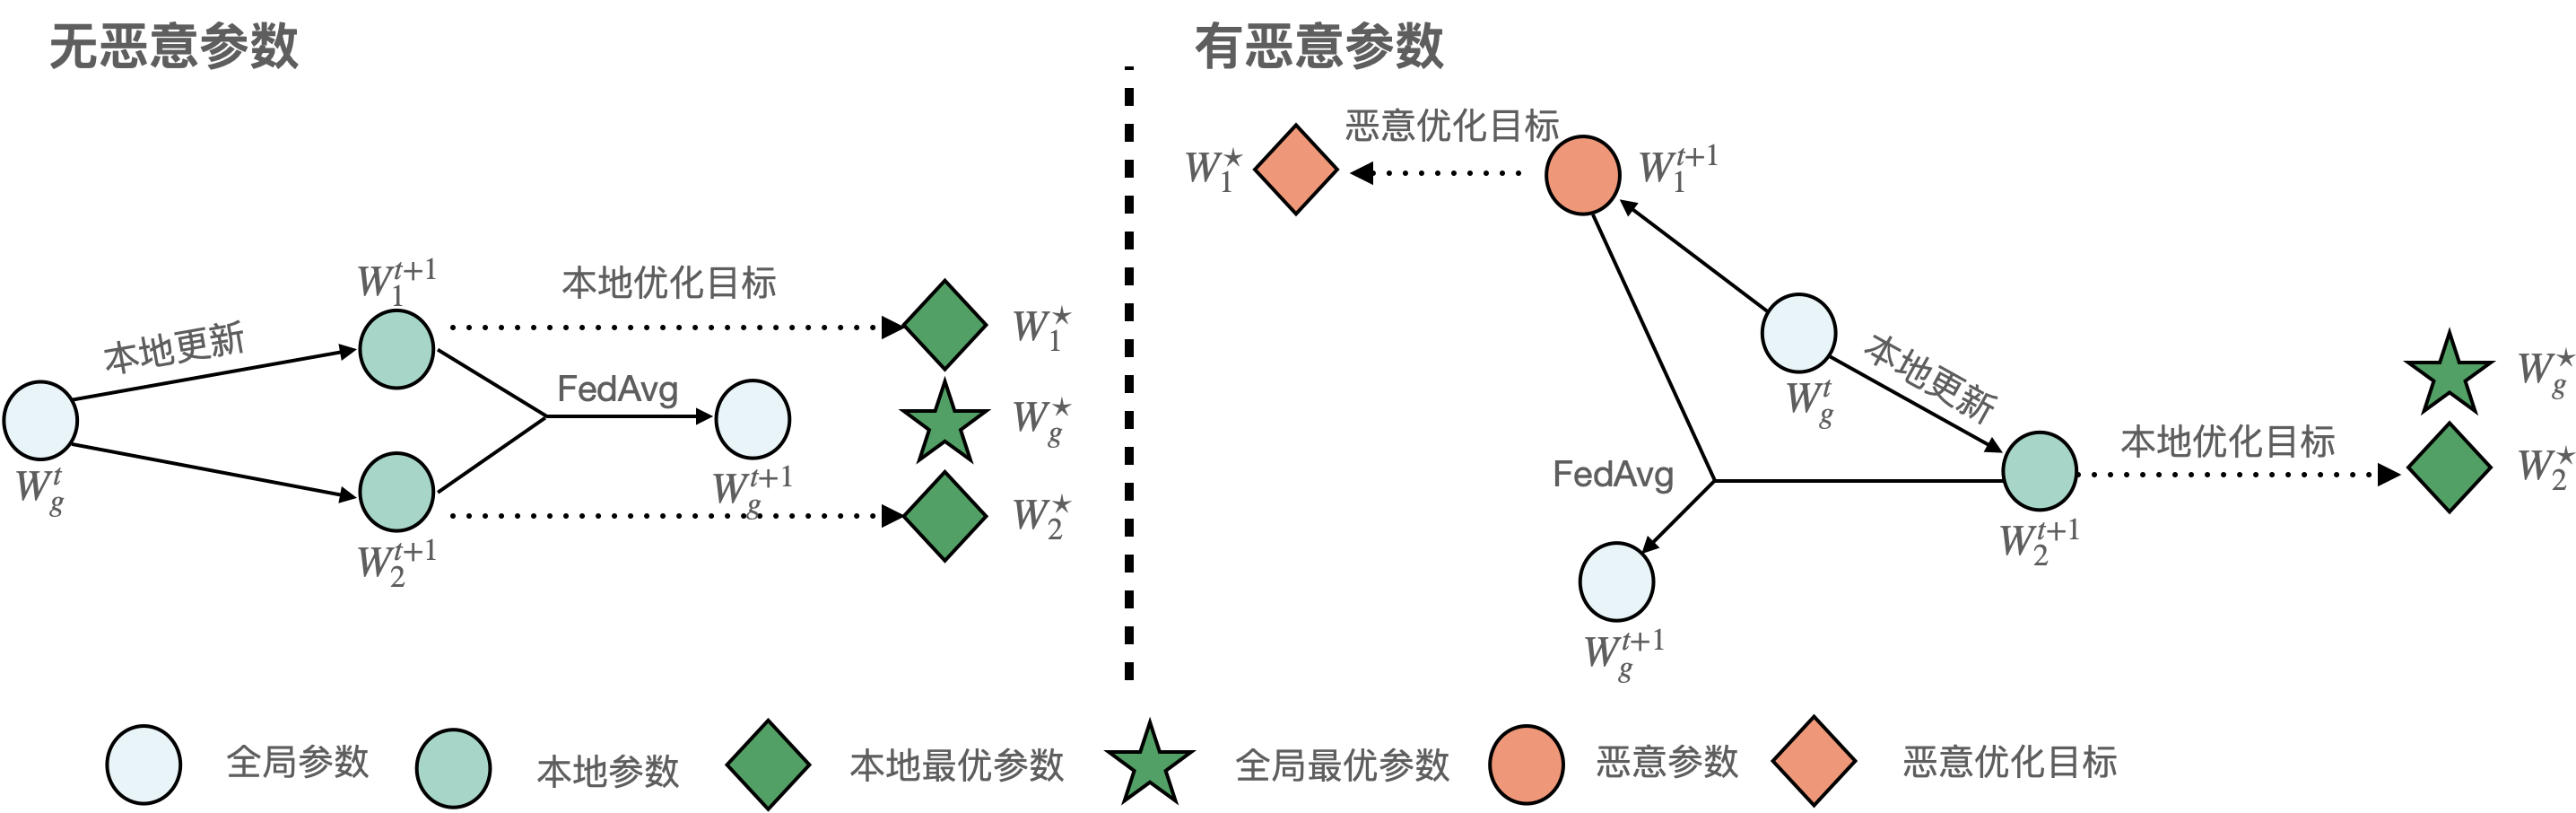
\includegraphics[width=\linewidth]{拜占庭v2}
	\caption{拜占庭节点影响示例}
	\label{byzantine}
\end{figure}

\begin{figure}[htbp]
	\centering
	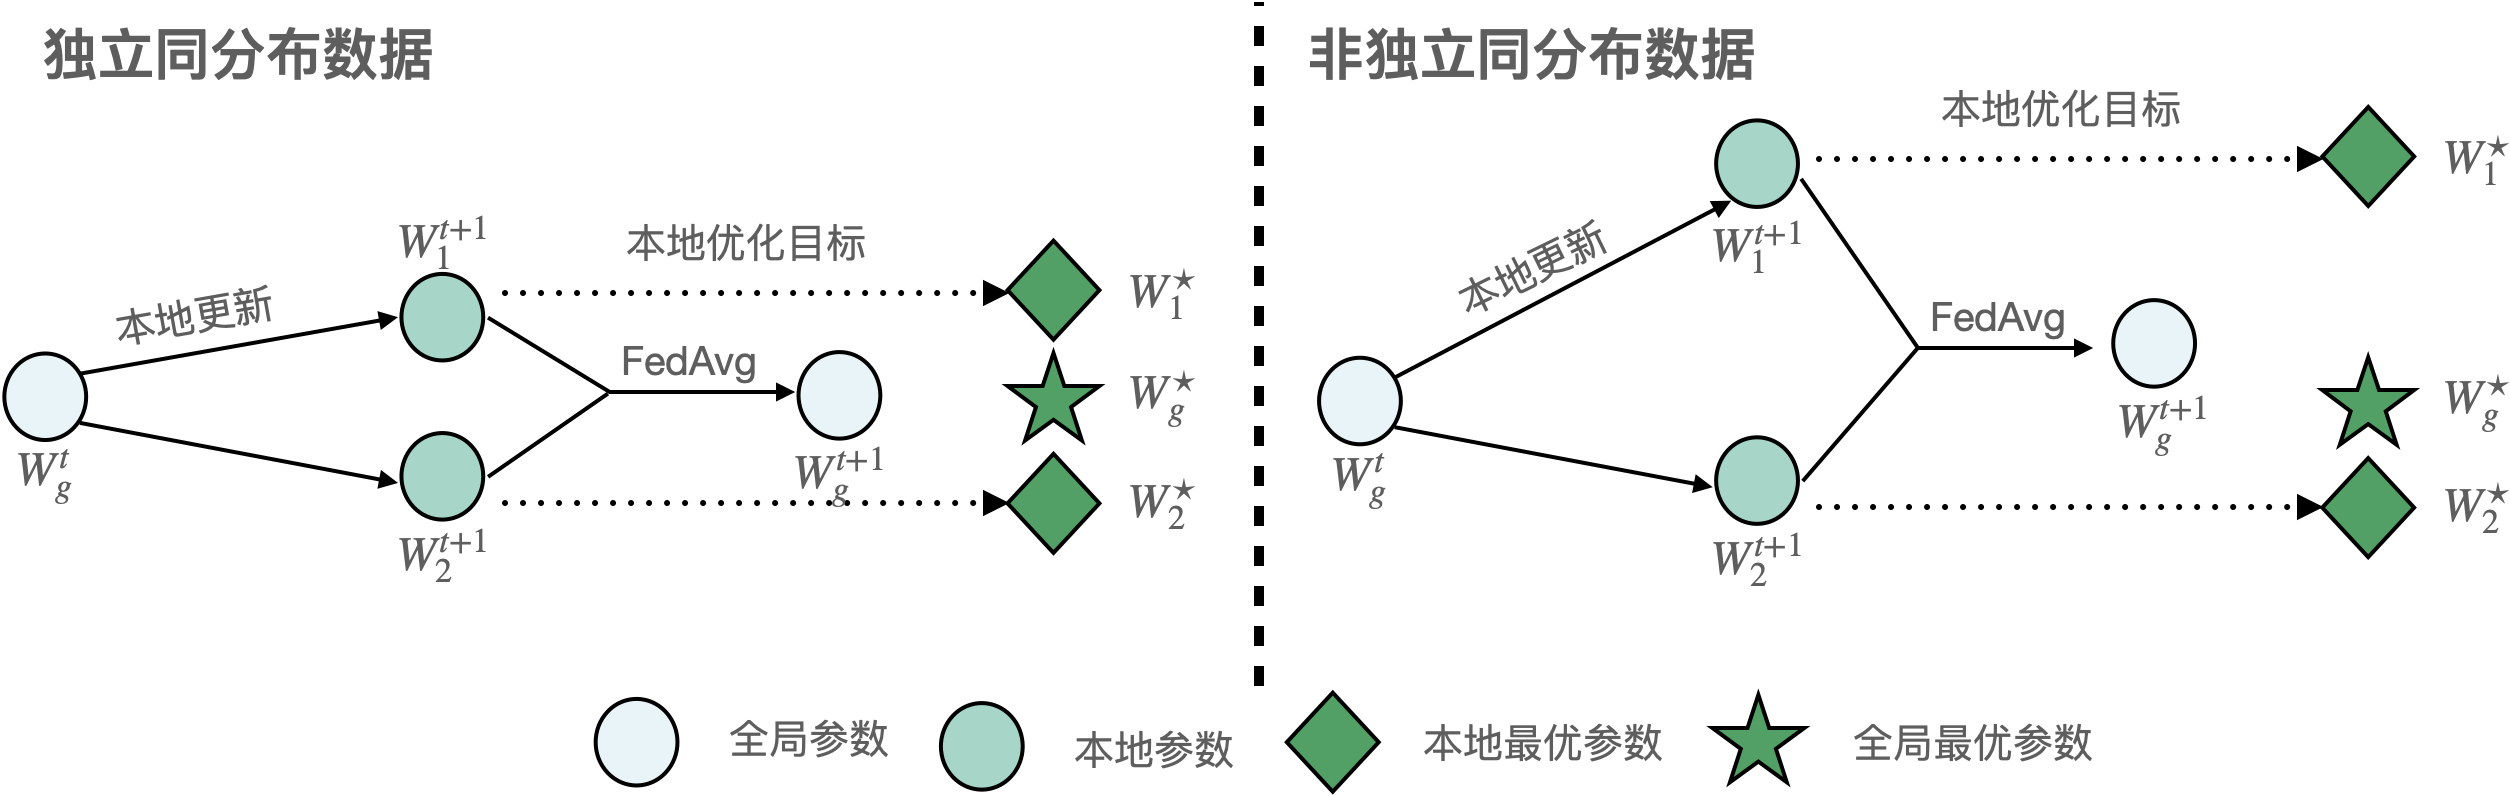
\includegraphics[width=\linewidth]{异质数据v2}
	\caption{异质分布数据影响示例}
	\label{non-iid}
\end{figure}

(2)异质分布数据的影响
%加图(那个实验性论文)

FedAvg算法非常适合不同参与方数据分布是独立同分布的场景,而相关研究\cite{zhao2018federated}表明,
异质分布数据会导致客户端之间的模型参数出现分歧,从而增加FedAvg算法的通信开销和收敛时间,同时也会降低FedAvg算法的全局模型的准确性和鲁棒性。

对于一些联邦学习场景,会出现不同参与方本地学习目标$F_k(W)$不一致的情况,在这种场景下使用FedAvg会逐渐加大参与方模型参数之间的差距,导致了最后全局模型推理准确率的低下。
图\ref{non-iid}展示了异质分布数据对于联邦学习的影响,对比独立同分布数据参与方相似的参数优化目标,异质分布数据的参与方的本地优化目标差距较大,FedAvg的聚合方式会让全局模型“走偏”,从而无法收敛到最优的全局参数。

上文提到的两种具体的联邦学习场景,都对FedAvg提出了挑战。
联邦学习迫切需要引入更加复杂的聚合权重分配方案,提升对于以上场景的鲁棒性。
同时,联邦学习也不能忽略对用户模型参数的隐私保护,这揭示了一个非常有挑战性的问题:
在隐私保护的限制下,寻求高效鲁棒的聚合方案,兼顾用户模型参数的\textbf{隐私性}、对具体场景的\textbf{鲁棒性}以及聚合算法的\textbf{高效性}。本文针对上述两种场景带来的挑战,分别提供对应的隐私、鲁棒以及高效的解决方案。
%因此需要考虑隐私、鲁棒以及效率三者之间的权衡,在保证用户隐私的前提下,设计高效鲁棒的聚合方案,以应对联邦学习中的复杂场景。

\section{本文研究内容和创新点}
%发现问题
%我们的方案,方案优点
本文立足于联邦学习中的模型参数隐私泄露问题,致力于在保证用户隐私的前提下,提升联邦学习在两种具体场景下的鲁棒性,即面对拜占庭节点的鲁棒性,以及面对异质分布数据的有效性,基于密码学理论构建并评估方案。

本文主要研究内容与创新点如下:

\subsection{面向拜占庭容错的模型参数安全聚合技术}
本文对联邦学习中的隐私保护问题和拜占庭节点问题进行了详尽的研究,发现目前的方案存在如下的局限性:$(\rm \romannumeral1)$没有兼顾模型参数的隐私性和对拜占庭节点的鲁棒性。
%已有的隐私保护联邦学习方案没有考虑潜在的拜占庭节点威胁,在拜占庭攻击面前十分脆弱,一个拜占庭节点的存在就能破坏整个学习过程;
一些旨在提升模型参数隐私性的联邦学习方案,没有考虑潜在的拜占庭节点威胁,在拜占庭攻击面前十分脆弱,一个拜占庭节点的存在就能破坏整个学习过程;
一些拜占庭鲁棒联邦学习方案则没有兼顾到其中的隐私威胁,在半诚实的服务器面前,有直接泄露用户原始数据的风险,而数据一旦泄露将造成难以挽回的损失。
$(\rm \romannumeral2)$兼顾隐私和拜占庭鲁棒的方案在权衡隐私、鲁棒以及高效时,存在一定缺陷。同时解决这两个难题极具挑战性,一方面隐私保护需要对模型参数进行加密或者混淆,而另一方面拜占庭鲁棒聚合算法的复杂计算需求对密文下的计算可行性和计算效率带来了极大的挑战。

针对目前研究存在的问题,本文在模型参数隐私性和拜占庭鲁棒性之间架起了一座桥梁。
具体来说,本文提出了一种平衡模型参数隐私、拜占庭节点鲁棒性以及计算高效性的联邦学习方案。
在隐私方面,本文使用多方同态加密实现对模型参数的隐私保护。
在鲁棒性方面,本文基于良性模型参数之间的相似性在密文上构建拜占庭鲁棒聚合方案,其涉及到的计算轻量,对密文计算友好,且能抵抗典型的拜占庭攻击。
同时,本文对提出的方案进行了详尽的安全性和收敛性分析,在真实世界数据集上进行了实验评估,证明了方案在权衡隐私、鲁棒以及高效上的优势。

\subsection{面向异质分布数据的模型参数安全聚合技术}
本文对联邦学习中的隐私保护问题和异质分布数据问题展开了深入的研究,发现目前的方案存在如下的局限性:
已有研究提升异质分布数据训练性能的联邦学习方案,往往都忽略了对模型参数的隐私保护问题,而同时兼顾这两者的方案在隐私性和扩展性上有待提升。
联邦学习中的异质分布数据联合训练是一个比较开放的问题,其解决思路主要分为三类:基于数据、基于算法或基于聚类方法,前两者都是在用户本地进行调整,不涉及到隐私问题。
基于聚类的方案通过聚类操作将拥有相似训练目标的参与方划分为一个簇,联合簇内用户协同训练,可以与其它方案结合进一步提升联合训练性能,是一个极具扩展性的方案,但是此类型方案没有考虑对模型参数的隐私保护问题。

针对目前基于聚类的异质分布数据联邦学习方案中的隐私问题,本文提出了一种兼顾隐私与异质分布数据训练性能,且拥有高扩展性的联邦学习方案。
具体来讲,
首先,本文使用加性秘密共享来保护本地模型参数和全局模型参数隐私,结合伪随机生成技术减少其中一半的通信开销。
其次,本文设计了安全高效的欧氏距离计算和曼哈顿距离计算协议来加速安全的层次聚类过程。
最后,为了提高安全聚类过程的计算效率,本文观察到模型参数在聚类过程中的维度冗余,在聚类前对模型参数进行了随机降维操作,保证聚类精度的同时,大幅降低了计算和通信开销。
此外,本文对提出的方案进行了形式化的安全性分析,同时利用真实世界数据集对方案进行了有效性和效率评估,证明了方案在面对异质分布数据时的安全性和高效性。

\section{论文的组织结构}
围绕上文叙述的研究内容,全文共分为五章,其组织结构如图\ref{struct}所示。

\begin{figure}[htbp]
	\centering
	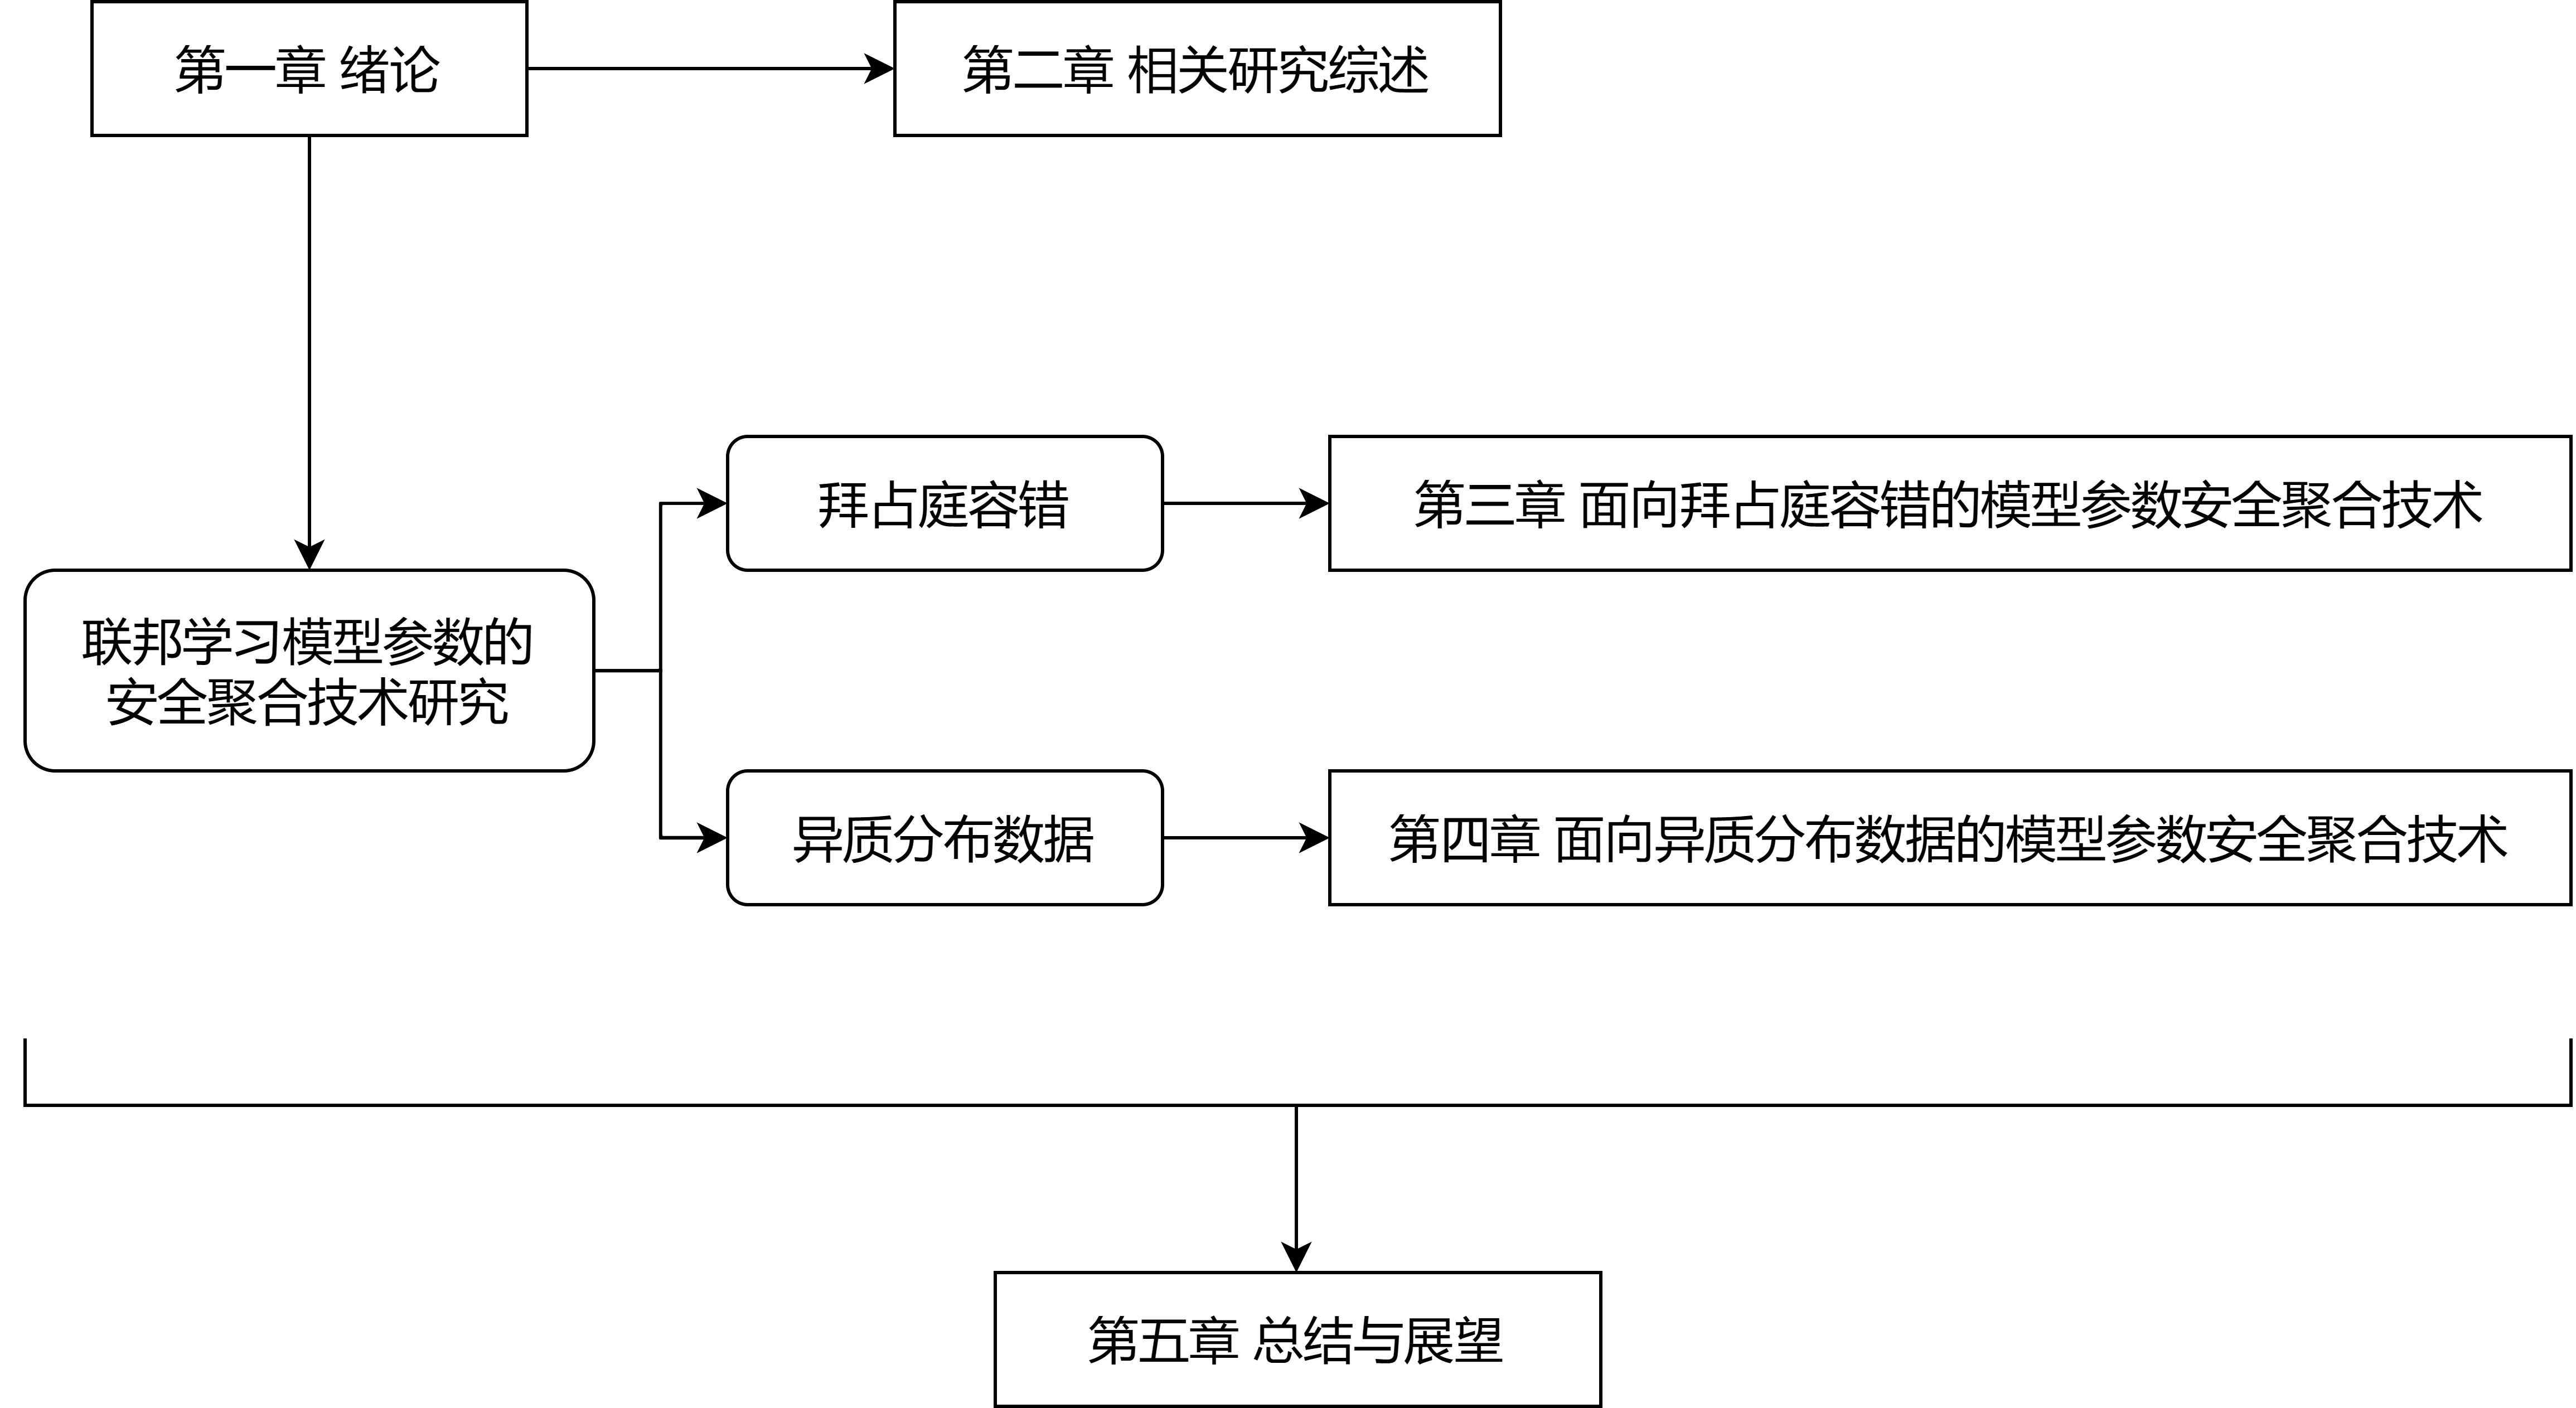
\includegraphics[width=0.9\linewidth]{论文组织结构v5}
	\caption{论文组织结构}
	\label{struct}
\end{figure}

本文的结构安排如下:

第一章为绪论。本章首先对本文的研究背景与意义进行了阐述,然后对于联邦学习以及其中的安全隐私问题进行了概述,最后介绍了本文的研究内容和创新点。

第二章为相关研究综述。本章对现有的研究方案进行了详细的调研与分析,主要展示了三个方面的研究:隐私保护联邦学习、拜占庭鲁棒联邦学习以及异质分布数据联邦学习。

第三章是面向拜占庭容错的模型参数安全聚合技术。本章针对联邦学习中的隐私威胁和拜占庭节点威胁进行研究,首先提出了一种密文计算友好的拜占庭鲁棒聚合算法,再利用多方同态加密构建隐私保护模块,实现了对模型参数的隐私保护、对拜占庭节点的鲁棒性以及计算的高效性,并通过理论分析和实验评估证明了方案的优势。

第四章是面向异质分布数据的模型参数安全聚合技术。本章针对异质分布数据对联邦学习带来的挑战进行研究,基于扩展性较好的聚类提升联合训练准确率的方案,利用秘密共享、伪随机生成等密码技术,高效实现了对模型参数的隐私保护,并通过理论分析和在真实世界数据集开展的实验,证明了方案在对模型参数提供强隐私保护的同时,实现了对异质分布数据联合训练准确率的提升。

第五章是总结与展望。本章首先对全文工作进行了总结,即本文提出的面向拜占庭容错的模型参数安全聚合技术,以及面向异质分布数据的模型参数安全聚合技术,然后对未来的工作方向和内容进行了展望。
